\documentclass{article}
\usepackage[utf8]{inputenc}
\usepackage[american]{babel}
\usepackage{csquotes}
\usepackage{hyperref}
\usepackage[backend=biber,style=numeric,hyperref=true,natbib=true,autocite=plain,sorting=none]{biblatex}
\usepackage[margin=1in]{geometry}

% this package and the below text is to force images to be added to the given section and subsection. See https://tex.stackexchange.com/questions/279/how-do-i-ensure-that-figures-appear-in-the-section-theyre-associated-with/235312#235312 for more information
\usepackage{placeins}
\let\Oldsection\section
\renewcommand{\section}{\FloatBarrier\Oldsection}

\let\Oldsubsection\subsection
\renewcommand{\subsection}{\FloatBarrier\Oldsubsection}

\let\Oldsubsubsection\subsubsection
\renewcommand{\subsubsection}{\FloatBarrier\Oldsubsubsection}

\addbibresource{references.bib}

\title{%
	NASA Suits Proposal \\
	\large Stevens Institute of Technology}

\date{October 2018}
\author{Joshua Schmidt, Ian Pizzolo, Ronnie Anker, Vincent Lee}

\usepackage{graphicx}

\begin{document}

\maketitle

\newpage

\tableofcontents

\newpage

\section{Letter of Intent}

\begin{center}

\bigskip
\bigskip
\textbf{Institution}
Stevens Institute of Technology
\bigskip

\textbf{Team Members}
\bigskip
\bigskip
\begin{tabular}{||c c c c||} 
 \hline
 Name & Email & Academic Year & Major \\ [0.5ex] 
 \hline\hline
 Ronald Ankner & \href{mailto:rankner@stevens.edu}{\nolinkurl{rankner@stevens.edu}} & Senior & Electrical Engineering \\ 
 \hline
 Vincent Lee & \href{mailto:vlee2@stevens.edu}{\nolinkurl{vlee2@stevens.edu}} & Junior & Computer Science \\
 \hline
 Joshua Schmidt & \href{mailto:jschmid3@stevens.edu}{\nolinkurl{jschmid3@stevens.edu}} & Sophomore & Computer Engineering \\
 \hline
 Ian Pizzolo & \href{mailto:ipizzolo@stevens.edu}{\nolinkurl{ipizzolo@stevens.edu}} & Sophomore & Mechanical Engineering \\
 \hline
\end{tabular}

\bigskip
\bigskip

\textbf{Advisor}
\bigskip
Mukundan Iyengar\newline
\href{mailto:miyengar@stevens.edu}{\nolinkurl{miyengar@stevens.edu}}\newline
\href{tel:12012165603}{+1 (201) 216-5603}

\bigskip
\bigskip
\textit{We plan to submit a proposal for the NASA SUITS Challenge.}

\end{center}

\newpage

\section{Introduction}

\subsection{Abstract}

\begin{figure}[!htb]
  \centering
  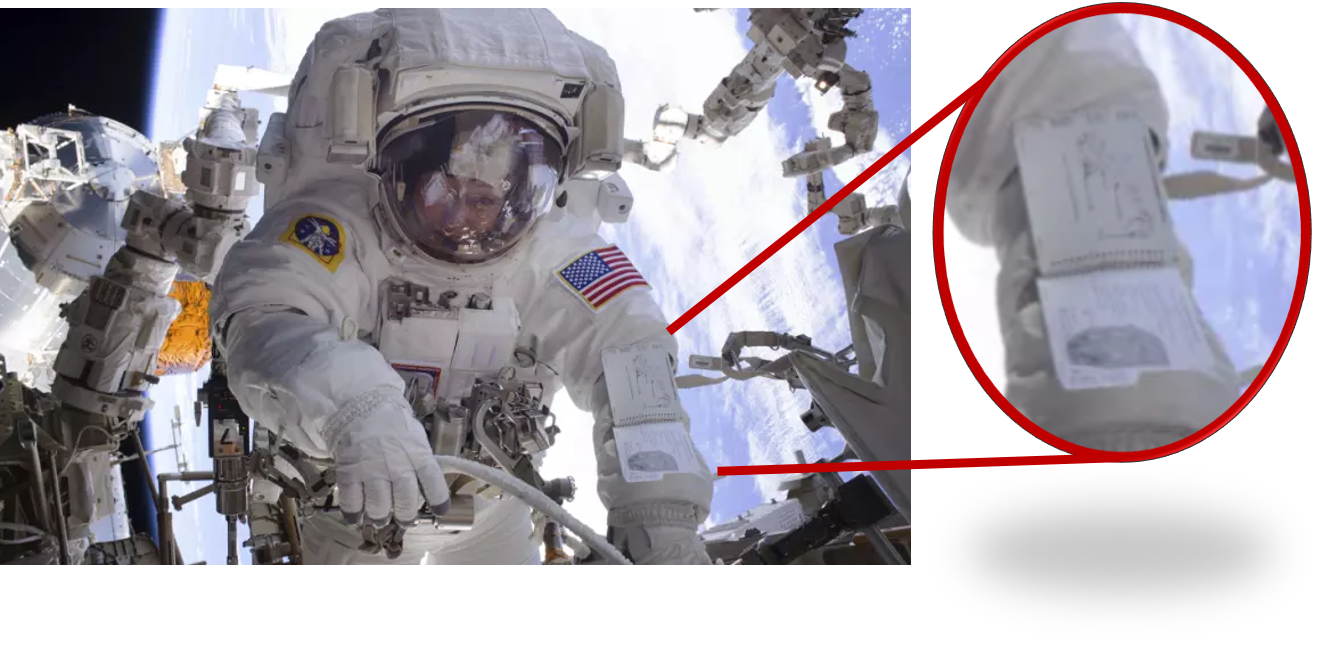
\includegraphics[width=0.75\textwidth]{assets/spacesuitdisplay.png}
  \caption{EVA Reference Notebook}
  \label{fig:spacesuitdisplay}
\end{figure}

The goal of our project is to aid astronauts on Extravehicular Activity (EVA) walks, which are activities or maneuvers performed by an astronaut outside a spacecraft. Currently EVAs are plagued by excessive amounts of information and minimal preparation time. During Gemini, Apollo, and the Space Shuttle era, specific space walks were heavily practiced prior to launch whereas now, the astronauts receive an EVA plan sometimes only a week prior to the walk \autocite{mannedspaceflight}. Moreover, astronauts no longer practice a specific EVA before launch, they prepare only generally for a multitude of possible EVAs. As shown in \textit{Figure \ref{fig:spacesuitdisplay}} due to the amount of planning and memorization needed, astronauts utilize notes for guidance. These notes are placed on the astronauts hand which can be inconvenient when they need to utilize both while still having access to the information written. Our goal for NASA SUITS is to remedy this archaic system and provide a solution that will reduce the minutia the astronaut has to worry about and allow them to focus on the main tasks of the EVA.

Our solution addresses these issues on two fronts. Employing a Microsoft Hololens, we plan to implement a heads up display paired with minimalistic display actuators for a more fluid interaction with external information. Moreover, we plan to implement image processing and localization tools in order to augment an astronauts environment, on command, and facilitate the astronauts actions. Our implementation includes 8 key functions:

\begin{enumerate}
\item Task Manager
\item Suit Status Manager
\item Handhold Helper
\item Inertial Monitor
\item “Way back home”
\item Caution and Warning System
\item Tool and Object Visualization
\item External Actuators, Inertial Measurement Unit (IMU), and Microprocessor
\end{enumerate}


\subsection{Design Description}

\subsubsection{Handhold Helper}

\begin{figure}[!htb]
  \centering
  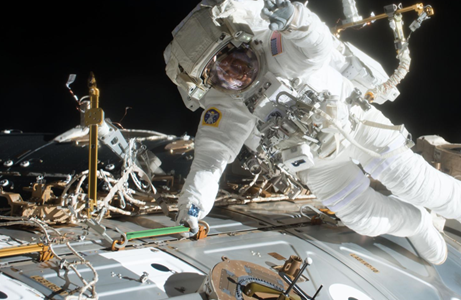
\includegraphics[width=0.75\textwidth]{assets/markedhandrail.png}
  \caption{Augmented Handhold Illumination}
  \label{fig:markedhandrail}
\end{figure}

As shown above in \textit{Figure \ref{fig:markedhandrail}}, the handhold helper will augment the astronauts perception by illuminating the next handhold to grab during his/her transit around the spacecraft. To achieve this, the system will employ both real time camera vision and known positions of various elements. Given the unique shape and distinct color of the handhold, the initial iteration of the camera vision algorithm will combine an edge detection element and a simple RGB threshold filter. If this proves not robust enough, the next iteration will emulate the Viola-Jones facial detection algorithm and utilize haar wavelets and training samples of handhold images in various orientations.

For positioning, the system will utilize the known positions of all handholds relative to spacecraft, the pre-planned progression of handholds provided in an EVA outline, and the known position of the astronaut relative to the spacecraft. The handhold positions and planned progression are assumed to be provided NASA prior to the EVA. The relative position of the astronaut will be supplied by our localization system, which will employ the Hololens built-in IMU and an external IMU that will interface with the Hololens. Using the known position of the next handhold relative to the spacecraft and the estimated position of the astronaut relative to the spacecraft, the position of the handhold relative to the astronaut can be found. Therefore, the estimated location of the handhold in the astronaut’s view is known and the handhold can be further discriminated via positioning.

Overall, our system will correctly discriminate the next handhold by filtering with edges, color, and position. The combination of this information will provide a robust method of determining the next handhold. With the handhold determined, the Hololens will then illuminate the handhold a distinct color, providing the astronaut an intuitive sense of which handhold to grab next.

Furthermore, in locating each handhold, the system can then compare its estimated position of the handhold within the astronaut’s view to the true position and back calibrate the relative positioning system. Assuming handholds will be relatively close, this allows for frequent error checking and calibration of the localization subsystem, preventing position estimation error from growing without bound.

\subsubsection{HandholdSuit Status and Task Manager}

\begin{figure}[!htb]
  \centering
  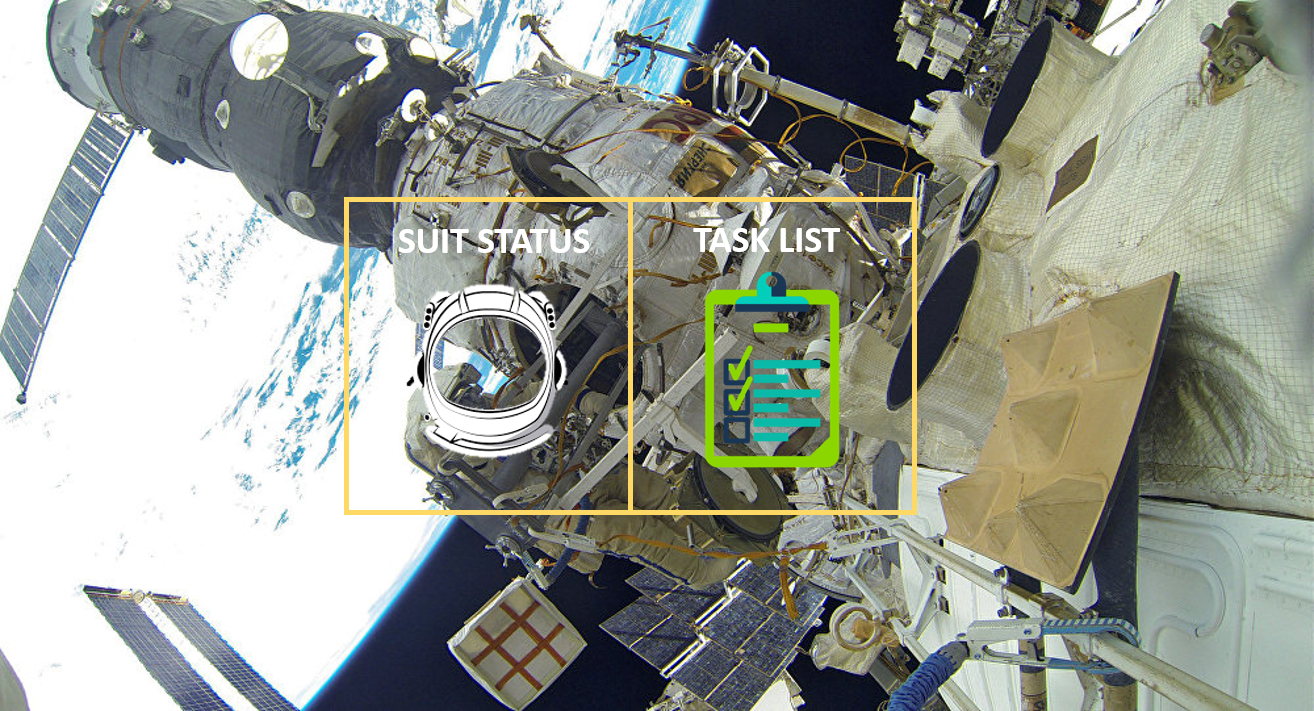
\includegraphics[width=0.75\textwidth]{assets/suitdatatasklist.png}
  \caption{Main Panel with Suit Status and Task Manager}
  \label{fig:suitdatatasklist}
\end{figure}

The main User Interface (UI) is intended to be as minimalistic and intuitive as possible; minimalistic so as not to detract from the astronaut’s field of view and intuitive to allow for quick and seamless use. On voice command, via the hololens and unity, the main panel displayed above in \textit{Figure \ref{fig:suitdatatasklist}} will appear. From this main panel, the astronaut can select between two options - suit status and task list. This selection will be done by physical actuators that the astronaut has located on the glove. The Suit Status displays all suit telemetry in a minimalistic manner, with an interface similar to \textit{Figure \ref{fig:moresuitmetrics}}. This data is mocked up and emulated for our use with a website that takes in data from a form and alerts the hololens and our program of the change to display. Showing our capability to dynamically change our information and eventually integrate with various endpoints to retrieve such information.

\begin{figure}[!htb]
  \centering
  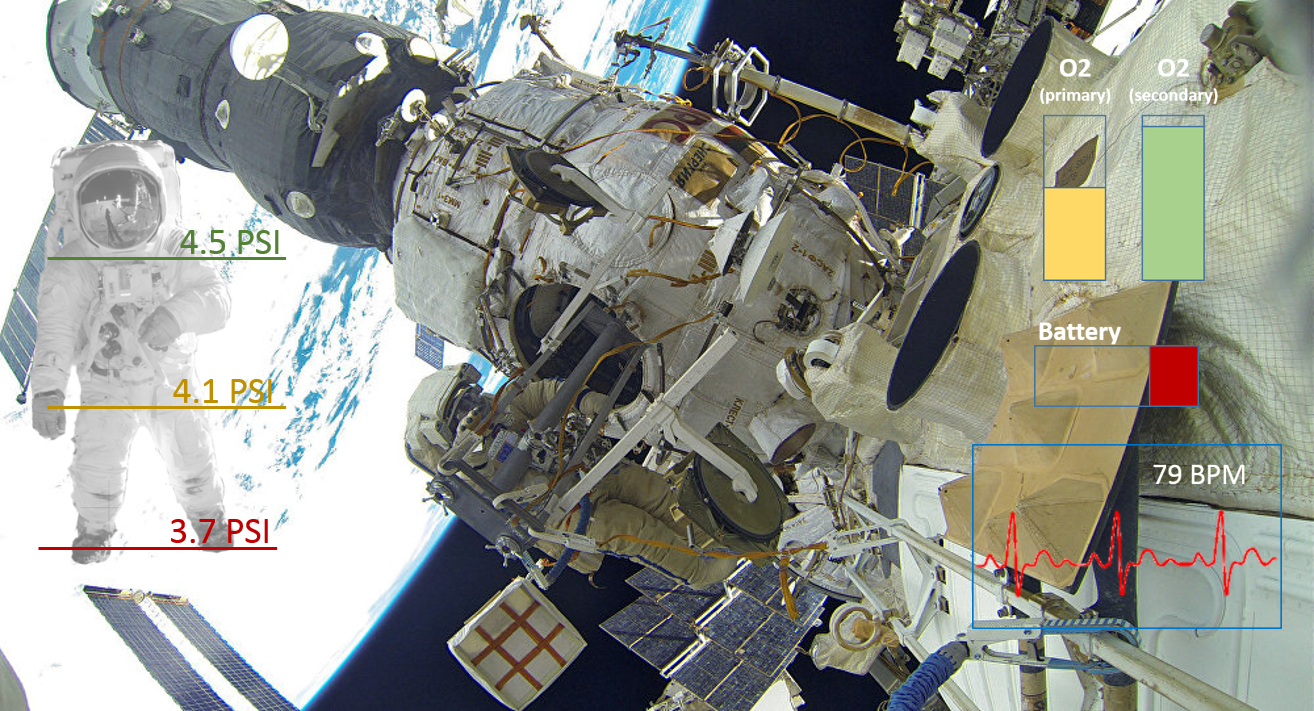
\includegraphics[width=0.75\textwidth]{assets/moresuitmetrics.png}
  \caption{Suit Status UI}
  \label{fig:moresuitmetrics}
\end{figure}

Again, this panel aims to maintain the astronaut’s field of view. Therefore, all metrics are placed outside of the astronaut’s main focus. The suit status panel shows the current suit pressure at differing regions, the astronaut’s heart rate, the current battery percentage, and oxygen levels. All metrics have intuitive indications of status: nominal operation in green, cautions in yellow, and warnings in red. For example, in the image above, battery level is dangerously low, primary O2 may require some attention, and secondary O2 is nominal. This color scheme will hopefully provide an intuitive sense of the suits status. The second panel, the Task Manager, displays the main task for the astronaut to complete \textit{Figure \ref{fig:task4}}.

\begin{figure}[!htb]
  \centering
  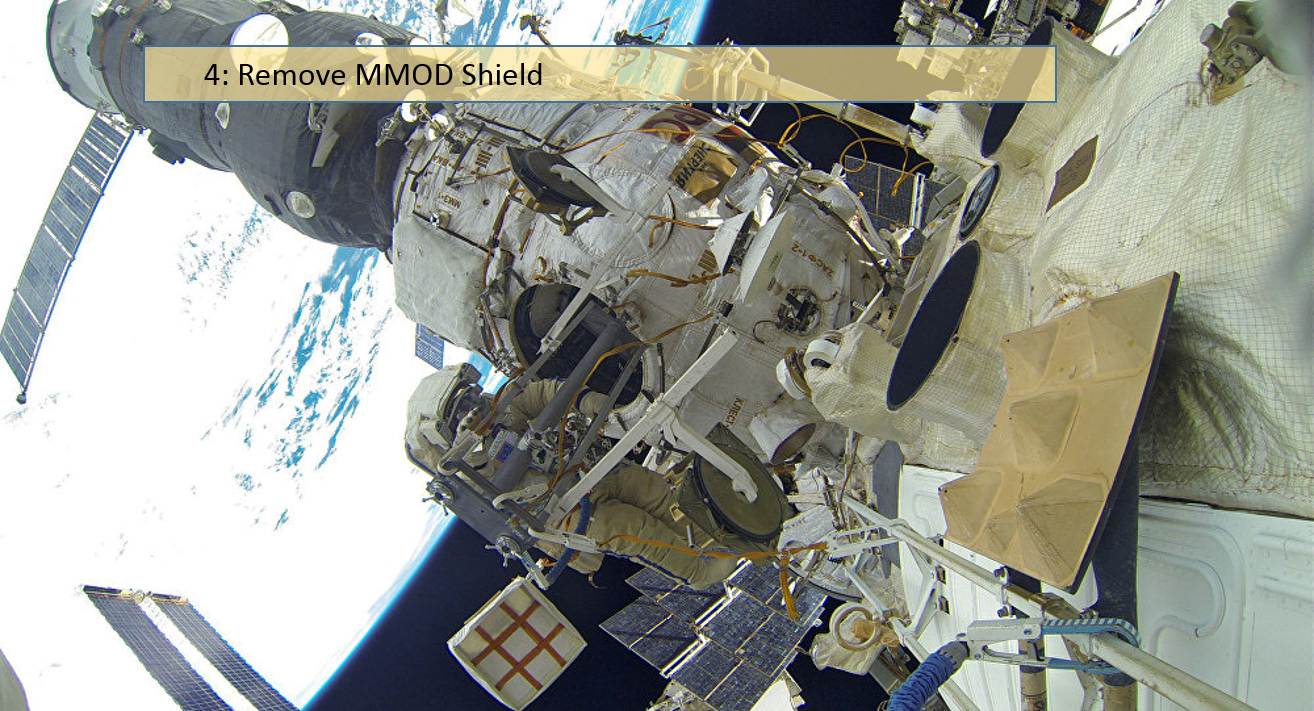
\includegraphics[width=0.75\textwidth]{assets/task4.png}
  \caption{Main Task UI}
  \label{fig:task4}
\end{figure}

The standard view is as shown above in Figure 5, where only the next major task of the EVA is displayed. If need be, the astronaut can access subtasks required to complete the main task via an actuator toggle (\textit{Figure \ref{fig:moresubtasks}}).

\begin{figure}[!htb]
  \centering
  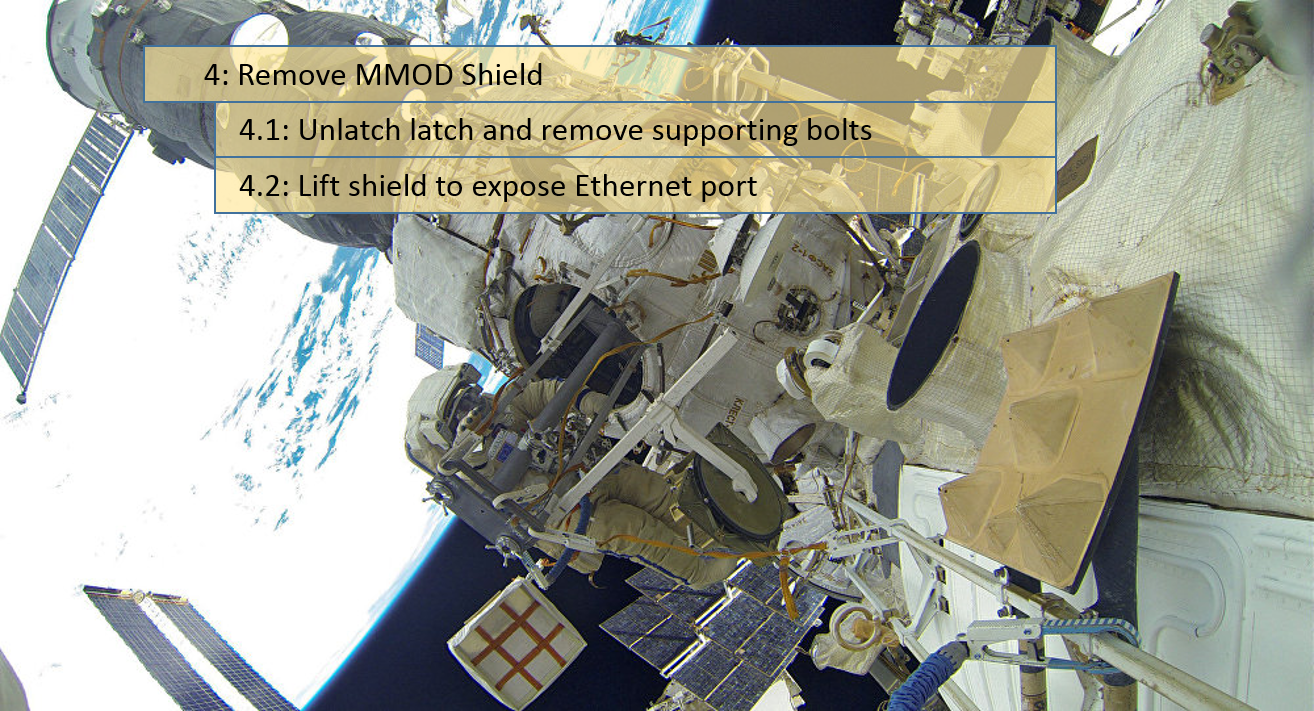
\includegraphics[width=0.75\textwidth]{assets/moresubtasks.png}
  \caption{Expanded Task View}
  \label{fig:moresubtasks}
\end{figure}

It is assumed that the tasks and subtasks will be meticulously prepared well ahead of the EVA, in which case all tasks and subtasks will be uploaded the the Hololens prior to the EVA. However, if and when plans change during the space walk, our system incorporates real time editing and addition of tasks and subtasks.

To input the tasks and subtasks for the prototype system, a progressive web application is used. It is currently hosted on Firebase but can be deployed anywhere, including on servers on the ISS, with slight modification. Tasks can be added in real time from multiple ground station nodes, and the webapp is updated in real time as well. This way both the astronaut and the ground station see the most up-to-date tasks and subtasks at all times. Additionally, the space suit sends sensor data and metrics to the webapp so the ground station can monitor the integrity of the suit. See \textit{Figure \ref{fig:taskmanagment}} and \textit{Figure \ref{fig:subtask}} for the user interface of the web application (\href{https://spacesuit.site}{spacesuit.site}). See the github repo for the source code (\href{https://github.com/jschmidtnj/spacesuits}{@jschmidtnj.SpaceSuits}).

\begin{figure}[!htb]
  \centering
  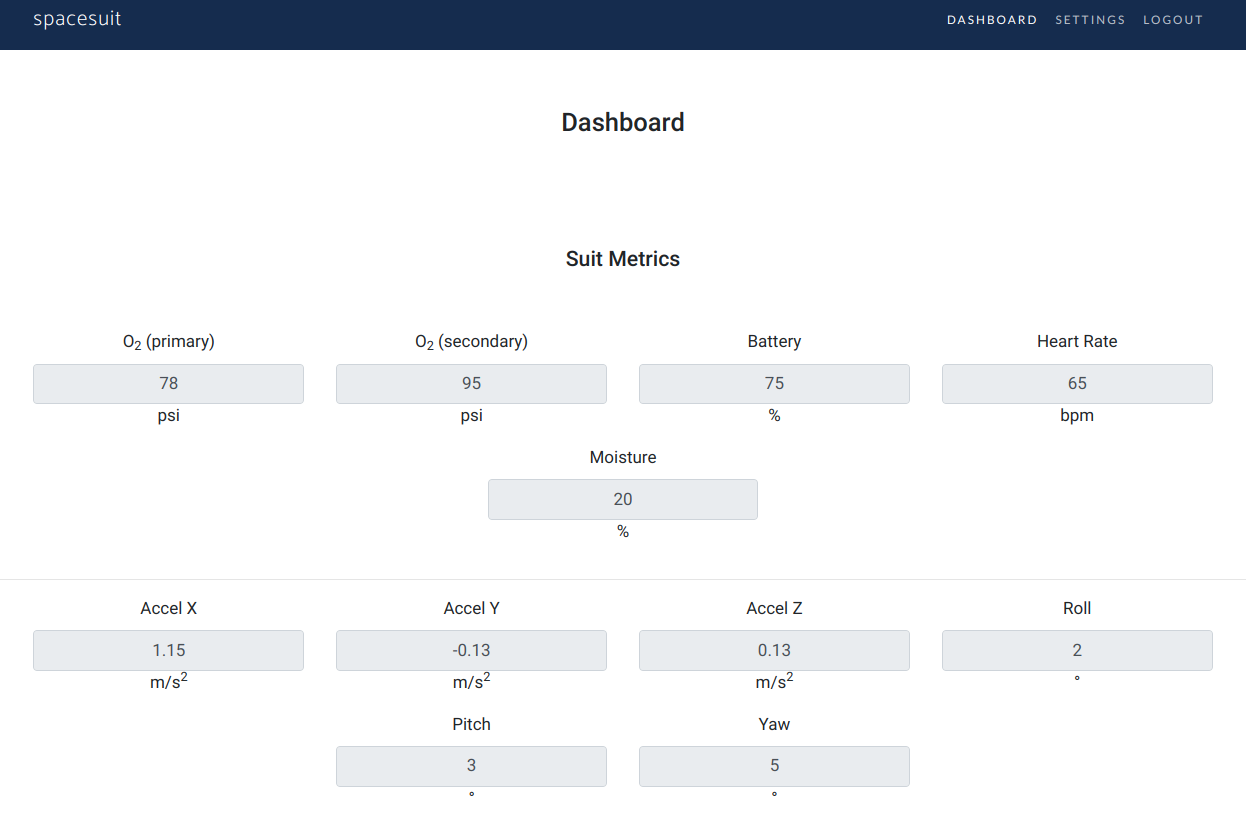
\includegraphics[width=0.75\textwidth]{assets/groundcontrolsuitmetrics.png}
  \caption{Suit Metrics Panel}
  \label{fig:groundcontrolsuitmetrics}
\end{figure}

\begin{figure}[!htb]
  \centering
  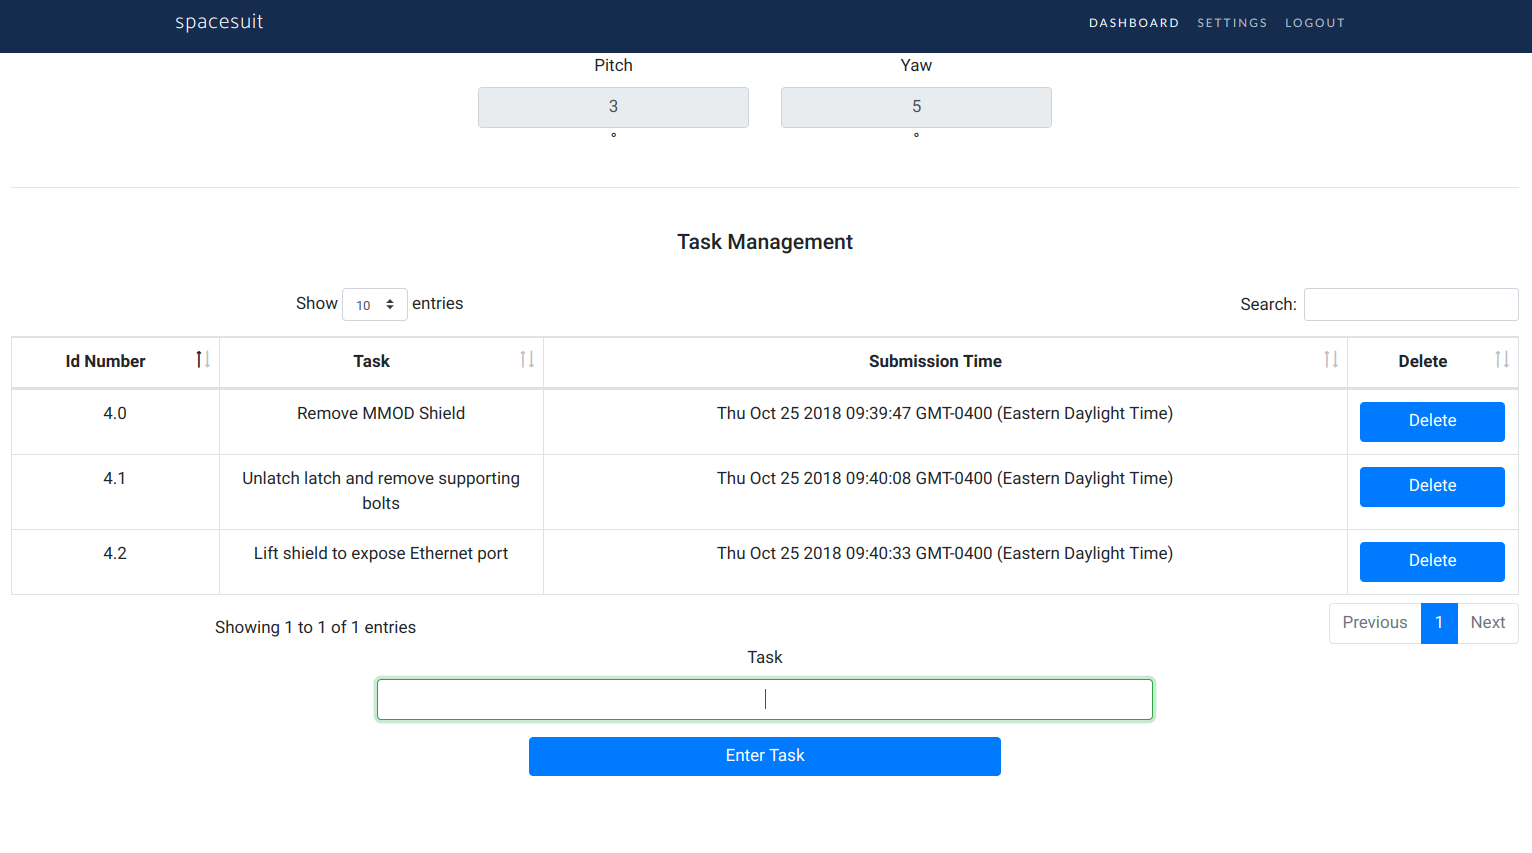
\includegraphics[width=0.75\textwidth]{assets/taskmanagment.png}
  \caption{Task Entry and View Panel}
  \label{fig:taskmanagment}
\end{figure}

\begin{figure}[!htb]
  \centering
  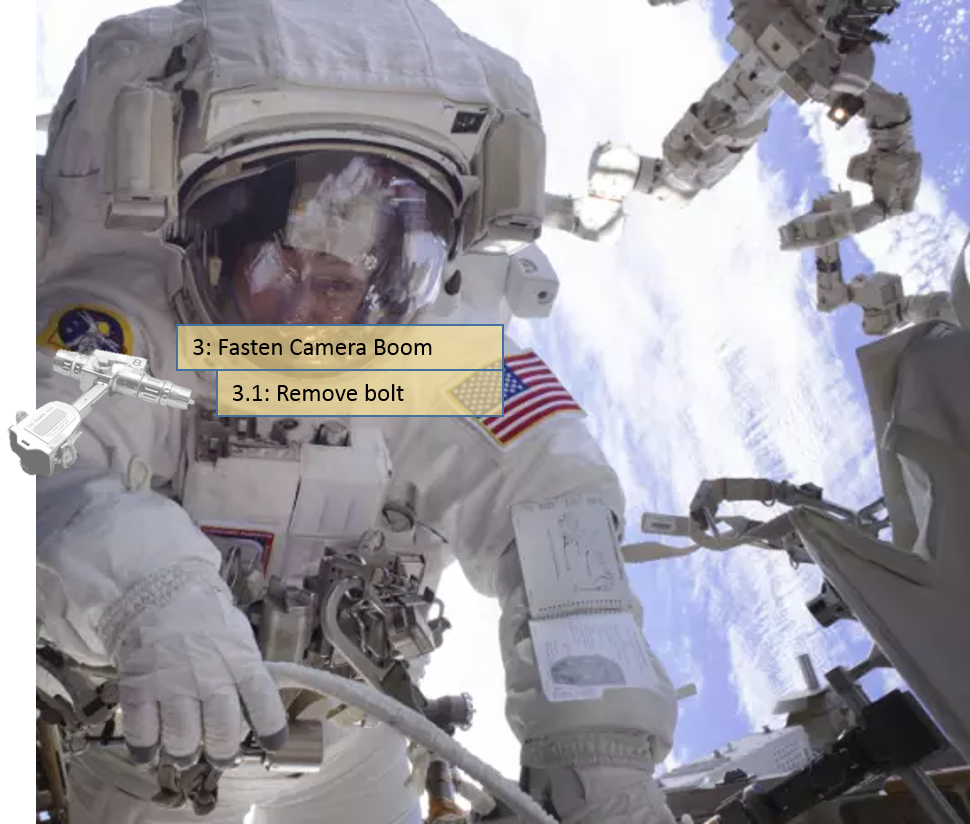
\includegraphics[width=0.75\textwidth]{assets/subtask.png}
  \caption{Tool and Object Visualization}
  \label{fig:subtask}
\end{figure}

Displayed above in \textit{Figure \ref{fig:groundcontrolsuitmetrics}} is an optional addition to the Task Manager. If a task requires the use of an uncommon tool or manipulation of an unusual object, the astronaut has the option of toggling the appearance of this tool next to the task manager. It is assumed that the CAD files any of these tools or objects in question will be uploaded to the Hololens well before the EVA and appear only on command from the astronaut via peripheral actuation.

\subsubsection{Inertial Monitor Panel}

\begin{figure}[!htb]
  \centering
  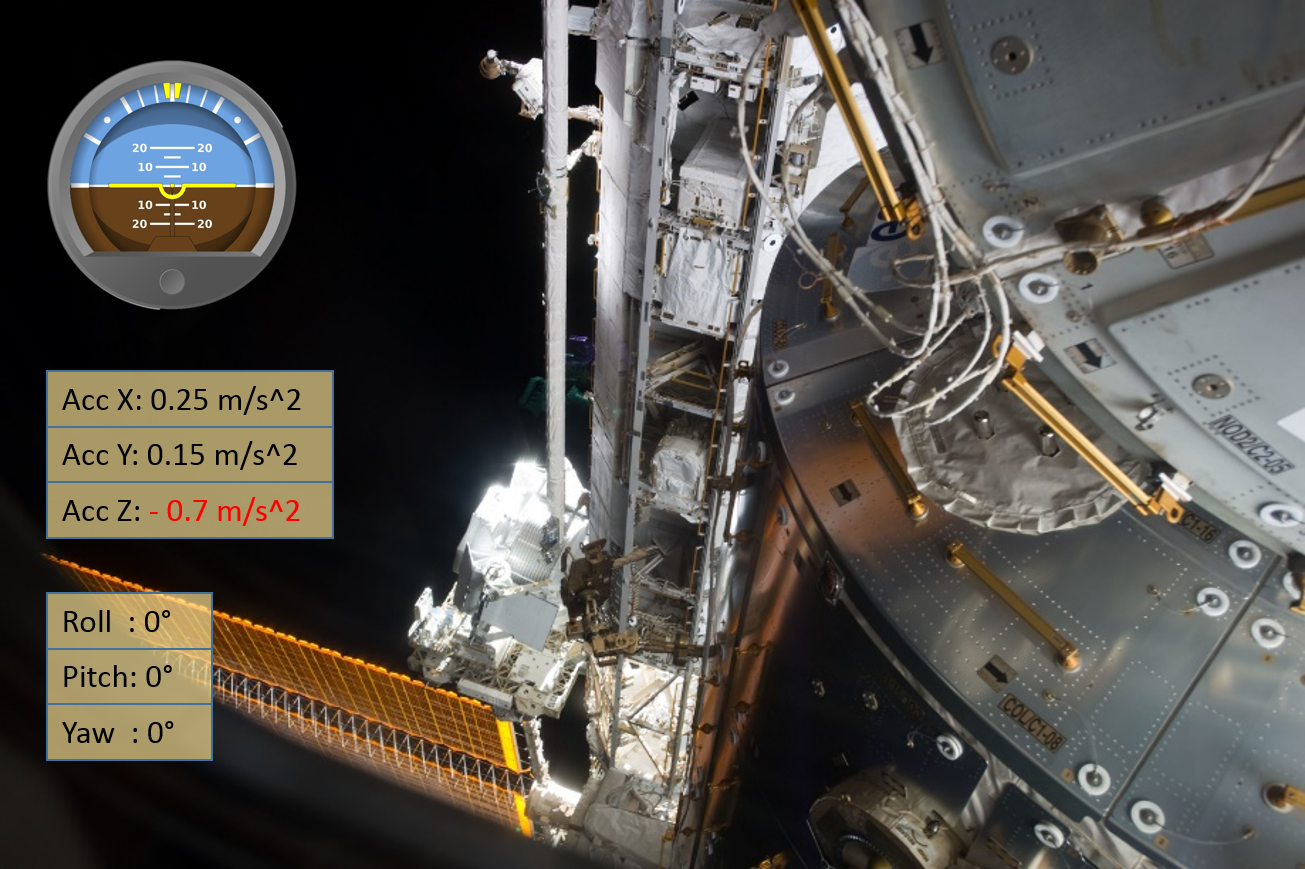
\includegraphics[width=0.75\textwidth]{assets/suitmetrics.png}
  \caption{Inertial Monitor Panel}
  \label{fig:suitmetrics}
\end{figure}

The inertial monitor as shown above in \textit{Figure \ref{fig:suitmetrics}} will provide a simple way to view the current inertial status. This panel will be used primarily for displaying warnings regarding the inertial data, for example if the astronaut is accelerating too significantly in any given direction as shown in \textit{Figure \ref{fig:suitmetrics}} by the “Acc Z” in red.  This panel can also be accessed via voice command by the astronaut. The inertial data for this panel will be provided by both the Hololens internal IMU and an external IMU we will be incorporating into our system.

\subsubsection{Way Back Home}

\begin{figure}[!htb]
  \centering
  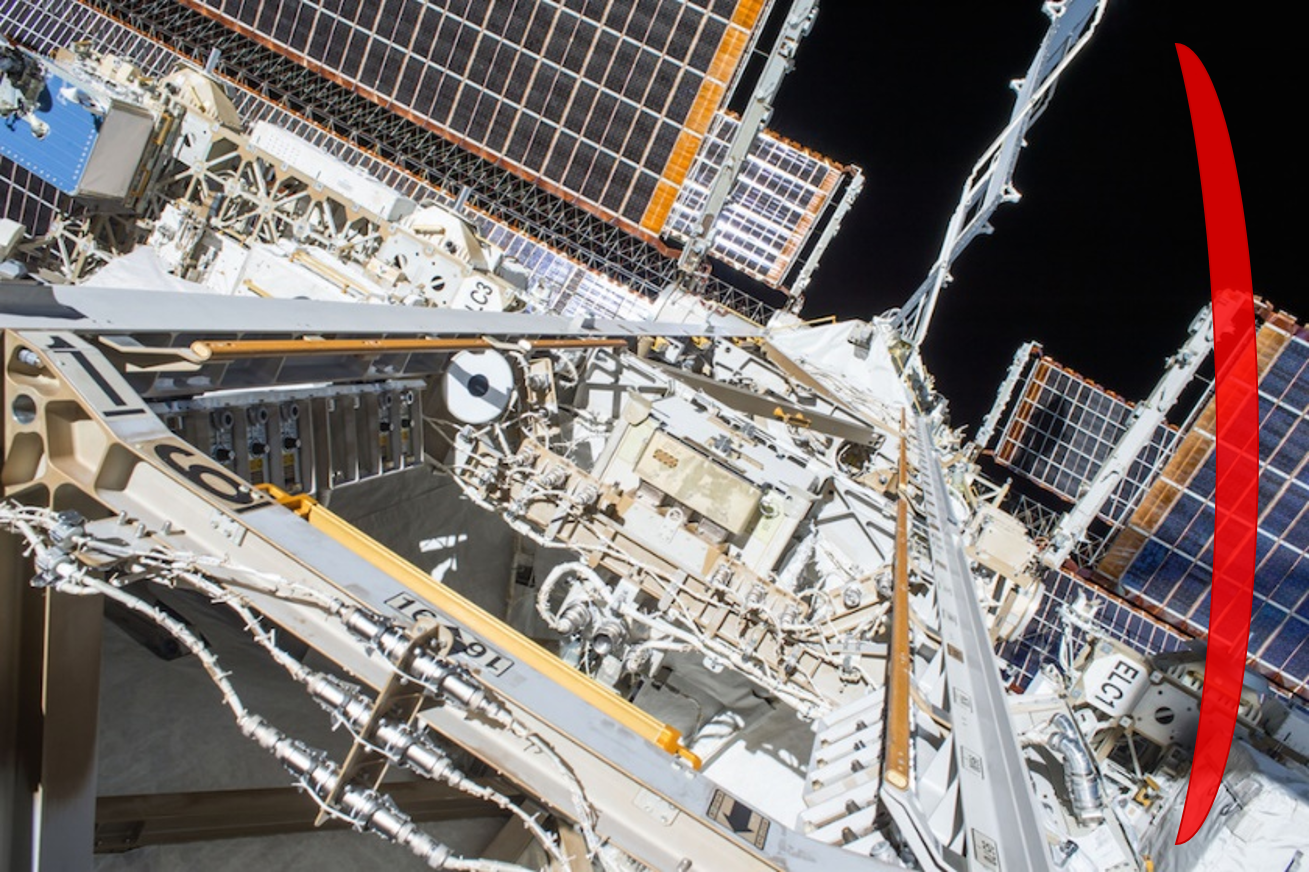
\includegraphics[width=0.75\textwidth]{assets/wayhome.png}
  \caption{“Way Back Home” Direction Indicator}
  \label{fig:wayhome}
\end{figure}

The “Way Back Home” \ref{fig:wayhome} will appear only in emergency situations. The system will continuously keep a position relative to the spacecraft access point. In times of emergency when an astronaut must get inside the spacecraft as quick as possible, this panel will appear and display a red indicator as shown in \textit{Figure \ref{fig:wayhome}} pointing toward the access point: an arrow when the access point is in the field of view and a red crescent when not in the field of view. 

\subsubsection{Caution and Warning System}

The caution and warning system will continuously monitor various metrics and employ both audio and the panels above to convey the issues. The system will have two sets of thresholds for each metric being monitored: one for caution and one for warning. The metrics that the system will monitor are as follows:  all suit telemetry, all inertial data, and task addition and deletion. For the suit telemetry, all cautions will be displayed in yellow on the panel. A caution will not trigger the panel to appear, but audio will notify the astronaut of the caution. A warning will be displayed in red on the panel and will trigger the panel to appear automatically. The panel will also be accompanied by audio indicating the warning. For example, if primary or secondary O2 drops below a dangerous pressure, the Suit Status panel will appear and the O2 bar graphic will be displayed in red. The inertial data will follow similar operation: a caution will trigger audio only and a warning will trigger the panel to appear accompanied by audio. Thresholds for the inertial data will be set such that a warning occurs only if the astronaut seems to be out of control. The appearance of this panel will hopefully aid the astronaut in regaining control as he or she can now see which degrees of motion are unstable or too high. For the task manager, the addition or deletion of a task can be set to caution or warning at the discretion of the operator editing the tasks. A caution will be indicated with audio and a warning will cause the Task Manager panel to appear, displaying the updated main task and subtask-expansion where an addition or deletion has occurred.

\subsubsection{Physical Actuators, IMU, and Microprocessor}

In order to control certain aspects of the Hololens operation, Physical Actuators will be added to the gloves. The physical actuators will consist of four strain gauges located on the middle knuckles of four fingers of one hand (thumb, pointer, middle, and ring), as that is the point of maximum deflection. Different predetermined combinations of finger movements will correspond to different actions and the actuators will be activated only after voice command to prevent accidental control of the Hololens carrying out manual tasks. The strain gauge output will be connected to a microprocessor, such as an arduino uno or raspberry pi. An auxiliary IMU will also interface with the microprocessor to allow for more refined inertial data when combined with the built-in Hololens IMU. The microprocessor will then continuously communicate with the Hololens via a bluetooth dongle to provide a fully-embedded system which does not rely on external networks.

\subsection{Concept of Operations (CONOPS)}

The goal of this project was to create a user friendly interface to help facilitate astronauts actions on EVA walks. With handhold helpers that illuminate the correct sequence of transit between worksites, our goal of alleviating the amount of procedures that astronauts have to remember is accomplished. In practice we hope that astronauts will be able to rely on this system to get them around so that they can concentrate more on the overall goals of their missions than having a trivial tasks in the back of their minds. Accomplishing this through a edge detection and a RGB filter, we aim to provide this information with low latency compared to other more complex and time consuming methods.

With the advent of a display for suit telemetry we aim to help put astronauts’ minds at ease as they have full access to and can be aware of the conditions they are in. We hope they utilize as their one stop shop for getting important information without struggling to look for where it is. Mocking this up with dynamic data from a form was the best way to display this capability in real time.

The tasks list is one of the biggests advantages of moving to an augmented reality interface. With a heads up display (HUD) of current and planned tasks we hope to help astronauts have an easy to use and accessible hub to relieve the burden of trying to read the objectives of a mission on their hand and by doing so restricting the use of their body. This implementation as stated before is set up to be able to handle dynamic changes which gives them the opportunity to adjust mid mission and accomplish more on each excursion. This feature achieves the goal of aiding the astronauts in their tasks and helps reduce the stress in forcing oneself to remember important but small details.

The way back, inertial monitor, and warning system is our way of further making our system a command center for an astronaut. It helps aid the astronaut in coordinating himself in dangerous situations which, while prepared for, can be assisted using the system we propose.

Our physical actuators are the most optimal in this case in order to have the astronauts have an efficient way to communicate with the system while still allowing them full use of their hands. When deciding on the specific way to activate the device, hand gestures were also suggested but this system would be difficult for astronauts to use in space as placing a hand directly in front of the hololens would prove difficult when restricted by a spacesuit. String gauges on the other hand allow an astronaut to activate the commands while not in view of the hololens. The biggest benefit of string gauges is that they can be fine tuned to prevent accidental activations and only activate with specific positions.

\subsection{Human-in-the-loop (HITL) Testing}

\begin{enumerate}
\item Actuator Testing: The actuators will be tested with a group of randomly chosen students on campus for feasibility and user experience. The group of students will be asked to perform a variety of navigational tasks in a controlled test environment, including navigating between the menus in the user interface, selecting options for tasks, and viewing system diagnostics. The ability for test subjects to complete these tasks using the actuators, and any comments as to making the experience more intuitive, will be documented and extrapolated. The test subjects will be randomly chosen, with a mixed population to accommodate various hand sizes and other metrics.
\item Handhold Helper: The second test will involve the handhold helper functionality of the helmet. Randomly chosen test subjects will be asked to locate a handhold in a controlled environment using the AR system, and the ease in which this task is performed will be recorded.
\item Orientation Help: The third test will involve the orientation helper. A randomly chosen subject test group will move their heads around with the helper activated, and test how accurate the orientation guidance is. They will rate the experience on a scale.
\item Web User Interface: To test the ground control user interface, we will again utilize a randomly-selected pool of test subjects to complete certain tasks in the web interface. These procedures in the ground control app would include adding certain tasks for the astronaut to complete, and monitoring the suit metrics data. The ease of use for the website and possible additional features will be recorded.
\end{enumerate}

\subsection{Team Project Schedule}

\begin{figure}[!htb]
  \centering
  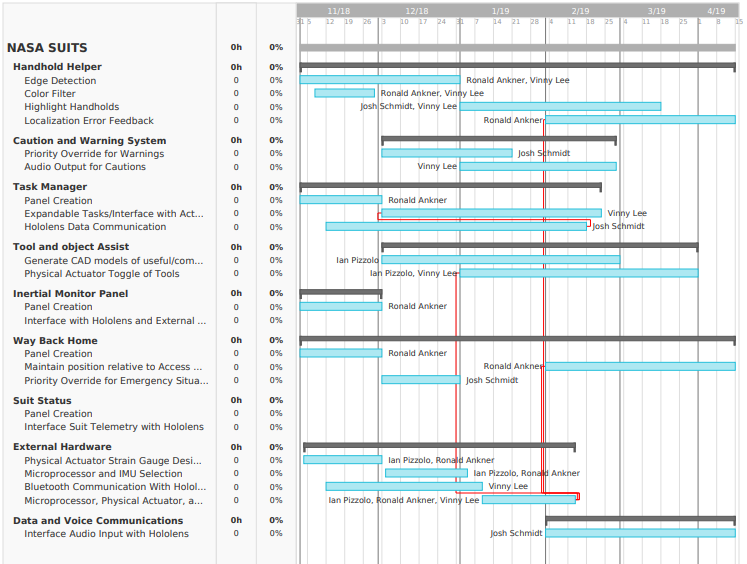
\includegraphics[width=0.75\textwidth]{assets/supertaskschedule.png}
  \caption{Schedule}
  \label{fig:supertaskschedule}
\end{figure}

\subsection{Technical References}

\printbibliography

\newpage

\section{Public Outreach}

Our plan with outreach is to spread the opportunities that NASA has such as competitions like this as well as potential careers and opportunities at NASA. Moreover, we plan on emphasizing the opportunities that STEM offers and how students can get exposure to it early. We plan on targeting high school and middle school students who have even a vague interest in STEM or space and aeronautics.

There are four groups we currently plan on visiting; Wayne Hills High School in Wayne, NJ, Hoboken High School in Hoboken NJ, Boy Scout Troop 130 in Wayne, NJ, and Raritan High School, Hazlet, NJ. As of now, we have one presentation confirmed at Wayne Hills High School for the spring (formal letter included at the end of the outreach section) and the other three are still developing.

Our presentation will follow a relatively similar layout, uniquely created by our team. The presentation will follow the below outline:

\begin{enumerate}
\item General Introduction What does STEM have to offer?
\item What NASA provides to the world
\item What NASA can provide to you
\item What you can provide to NASA
\item Personal STEM/NASA Experiences
\begin{enumerate}
\item Vincent Lee
\item Joshua Schmidt
\item Ian Pizzolo
\item Ronnie Ankner
\item Swag (from JSC Education Office and Public Affairs Office) and Questions
\end{enumerate}
\end{enumerate}

While each presentation will be slightly different, the general theme and key points (not word for word) are touched upon in the section below, accompanied by pictures we will likely show.

\subsection{General Introduction: What does STEM have to offer?}

Science, Technology, Engineering, and Mathematics, colloquially known as STEM, offers an unobstructed view into the universe. It provides a powerful method to understand and see the world around us, and better yet, manipulate it. STEM is what allows us to see thousands of galaxies billions of miles away and thousands of atoms that make up the head of a nail. It is what allowed humanity to first sail between the continents (and find our way back), to first take flight, to explore the cosmos and the secrets it holds. It allows us to cure diseases that plagued the human race  for centuries and give mobility back to those that have lost it. Overwhelmingly  though, STEM gives each and every one of us the power to change the world around us for the better.

\subsection{What NASA provides to the world}

\begin{figure}[!htb]
  \centering
  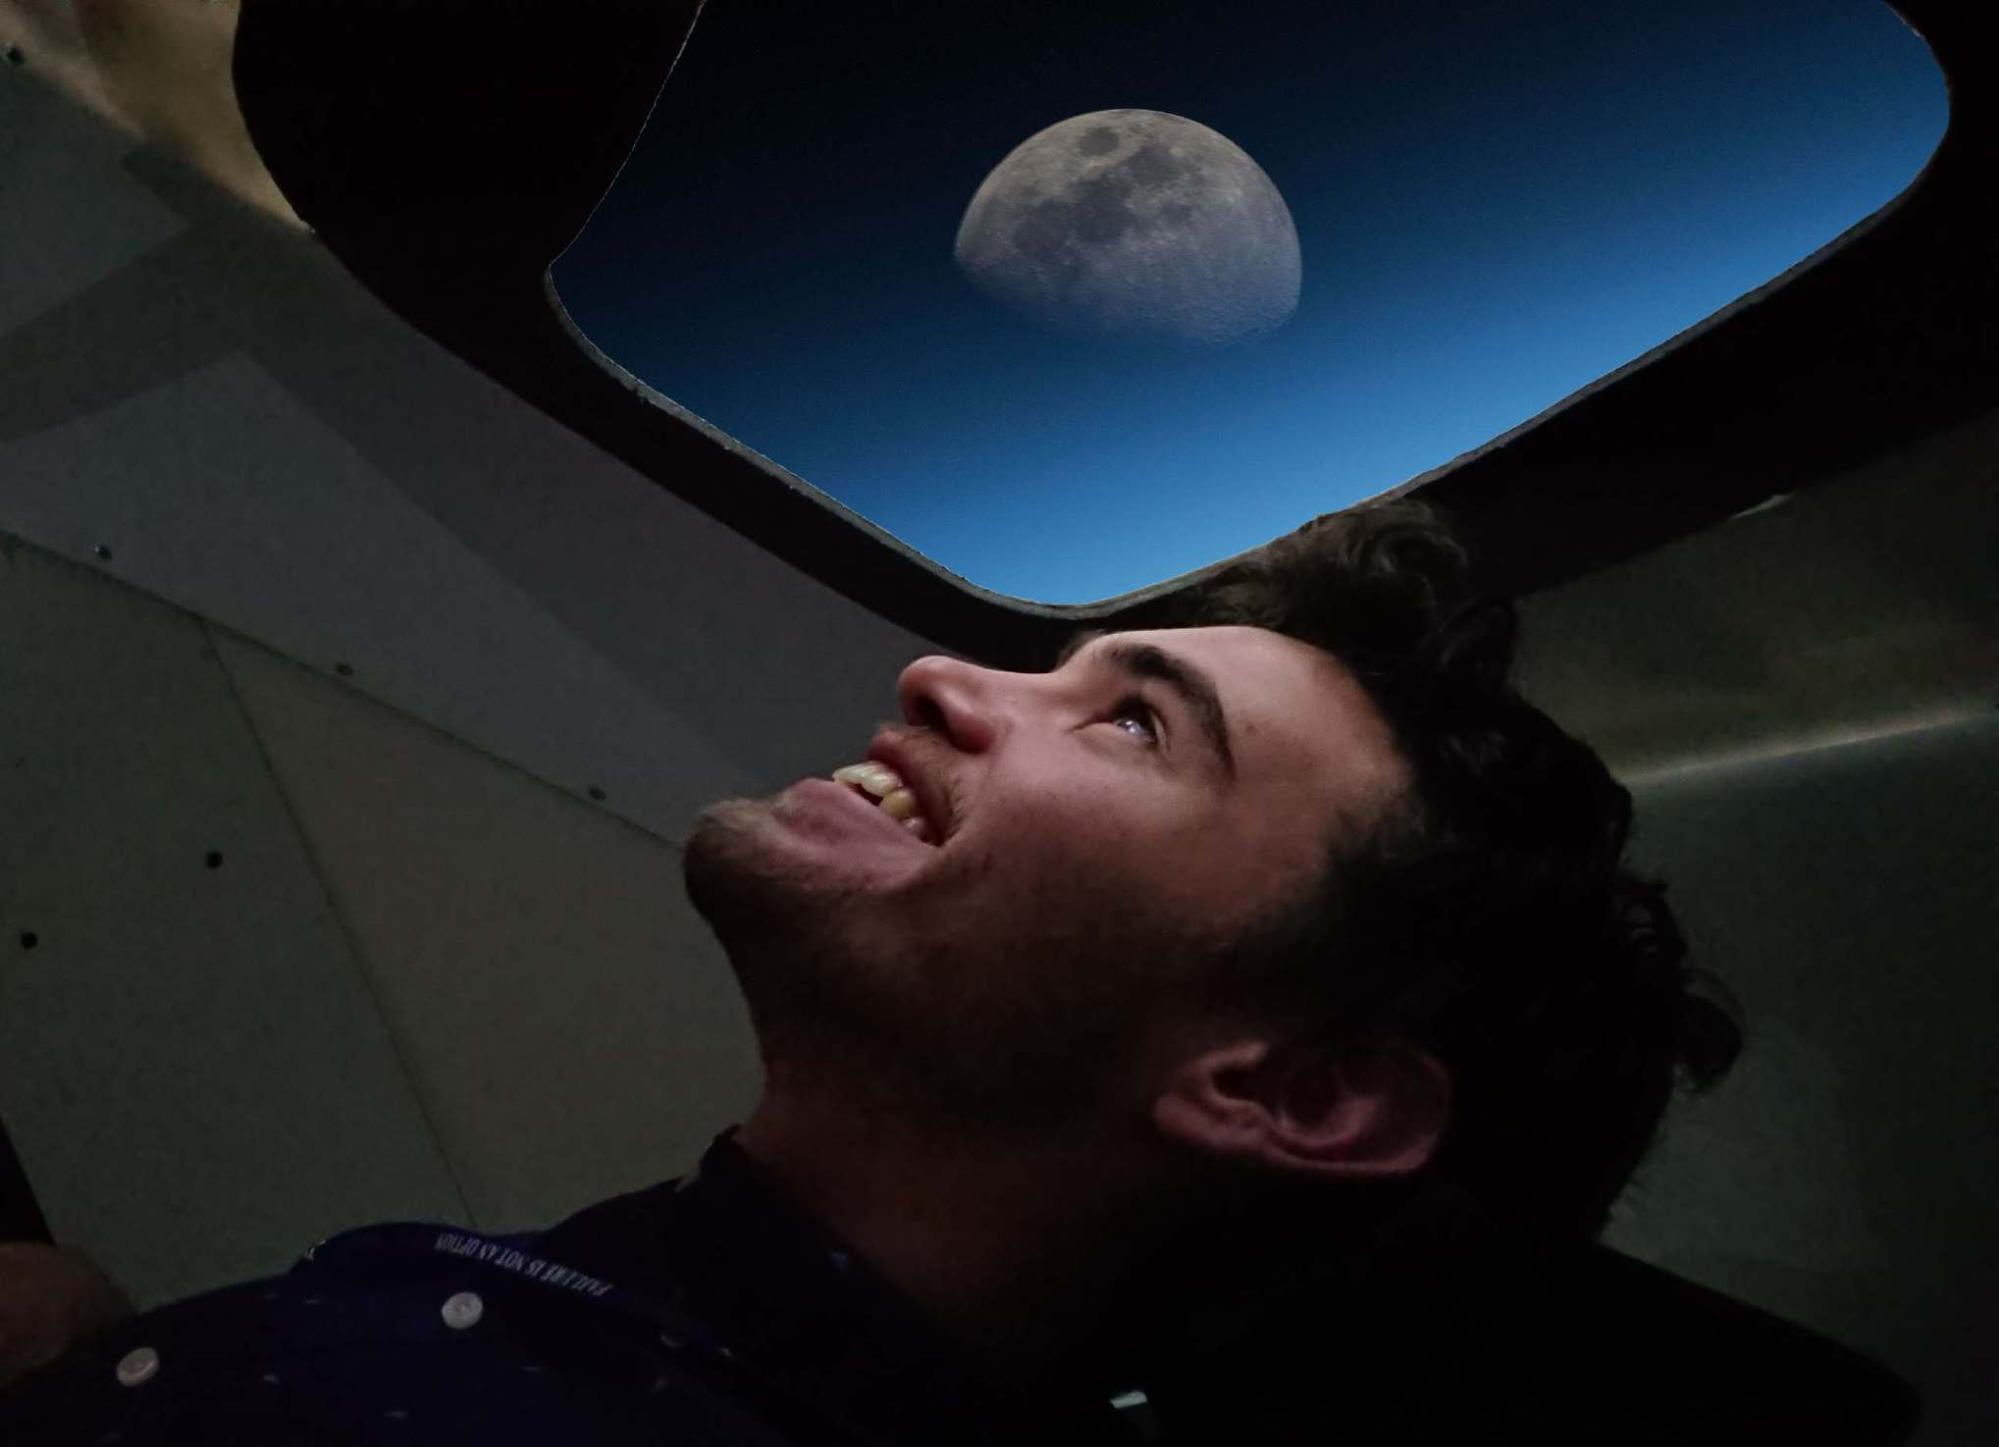
\includegraphics[width=0.75\textwidth]{assets/smilingatthemoon.jpg}
  \caption{Moon Shot}
  \label{fig:smilingatthemoon}
\end{figure}

For the last 60 years, above scientific advancement and community, NASA has provided inspiration to the world. Shortly after its creation, NASA was thrown into the kiln with one of the hardest problems humanity to that point had ever faced: putting humanity on the moon. With the time, sweat, and dedication of over 50,000 Americans and over the course of 7 years, NASA brought humanity to moon and with it ushered in a new era of human progression: transforming humans into a multi-planetary species. So influential was that step that now any task seemingly-impossible or any goal too lofty is often said to be a “moon shot”. That event and the work required to achieve it left an indelible mark on society and has been inspiring up and coming dreamers in every generation since, us included. 

Furthermore, NASA’s mission is the benefit of humanity, which is very quiet literally illuminated in its motto: “For the benefit of all”. With this mentality, hundreds of thousands of diligent employees have been working over the last 60 years to advance society in areas including, but most certainly not limited to, space, aeronautics, medicine, biology and the environment. NASA tackles the hardest problems of the time and moreover, outsources all of its discoveries. The work done, the research conducted, the discoveries made, all are done in the effort of advancing humanity.

\subsection{What NASA can provide to you}

Overall, working with NASA can provide great experiences, incredible applications in STEM, some of the hardest problems on and off this world, and more powerfully, a family. Below in \textit{Figure \ref{fig:bigoutreachgroup}} and \textit{Figure \ref{fig:smalleroutreachgroup}} are pictures taken of a lectures given my Apollo flight director Gene Kranz and current Astronaut Victor Glover to interns. Even as an intern, working at NASA can provide the opportunity to hear such influential and accomplished people as Gene Kranz and Victor Glover speak. Moreover, working at NASA can provide the opportunity to become those people.

\begin{figure}[!htb]
  \centering
  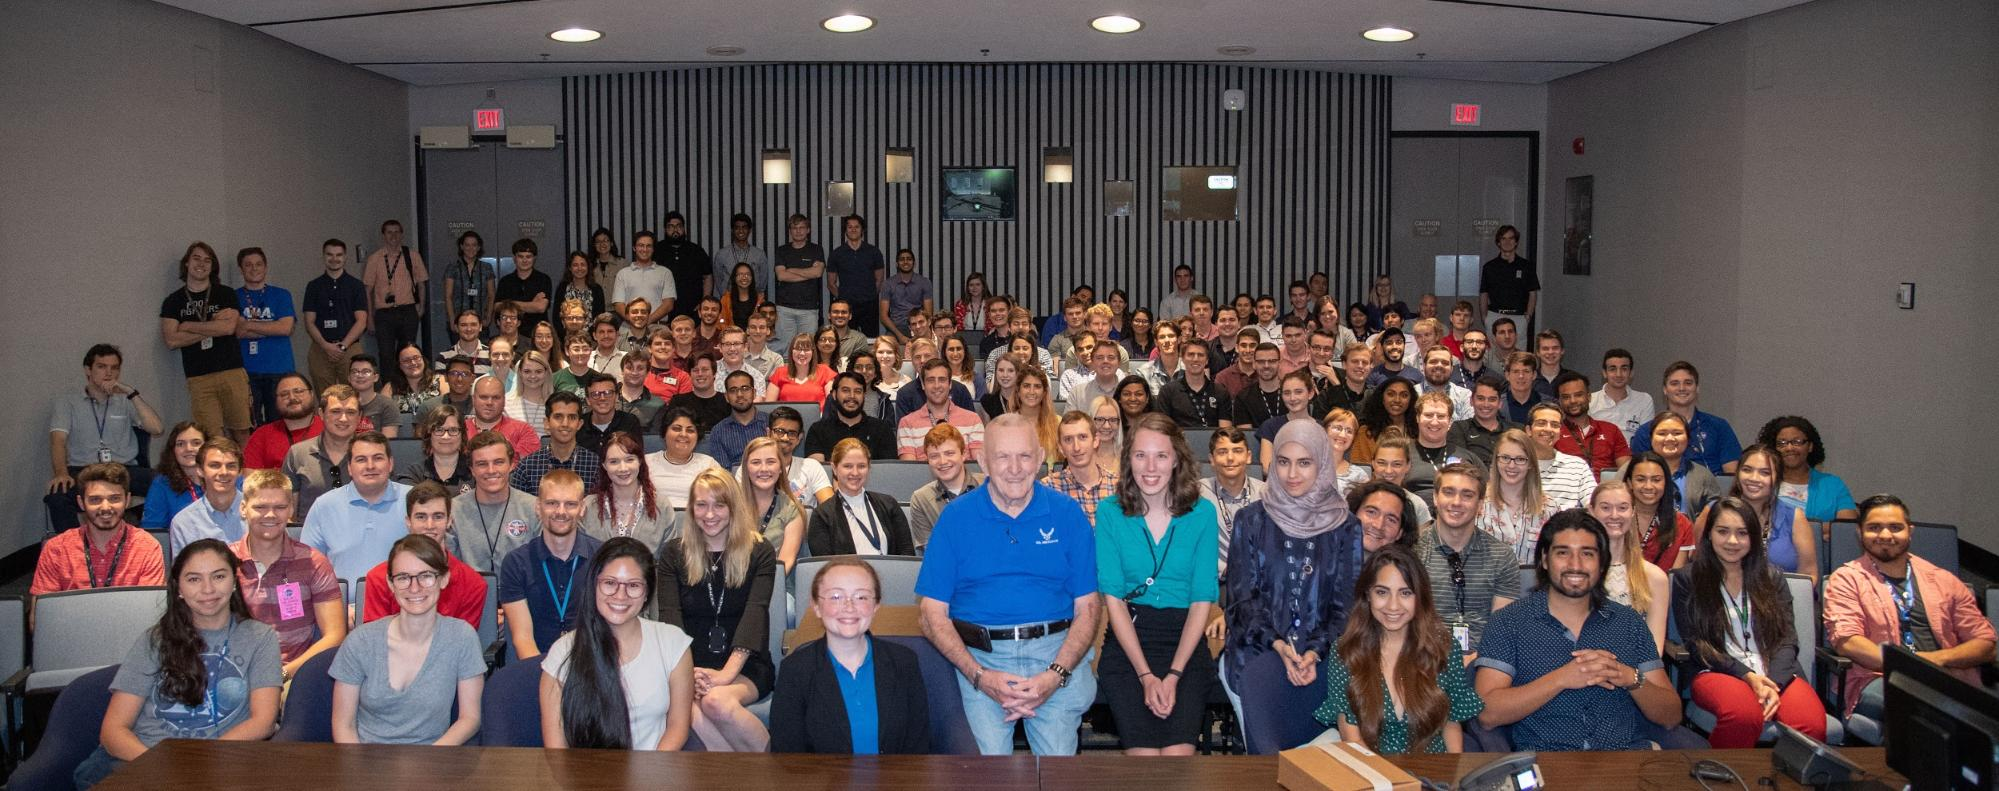
\includegraphics[width=0.75\textwidth]{assets/bigoutreachgroup.jpg}
  \caption{Gene Kranz Lecture}
  \label{fig:bigoutreachgroup}
\end{figure}

\begin{figure}[!htb]
  \centering
  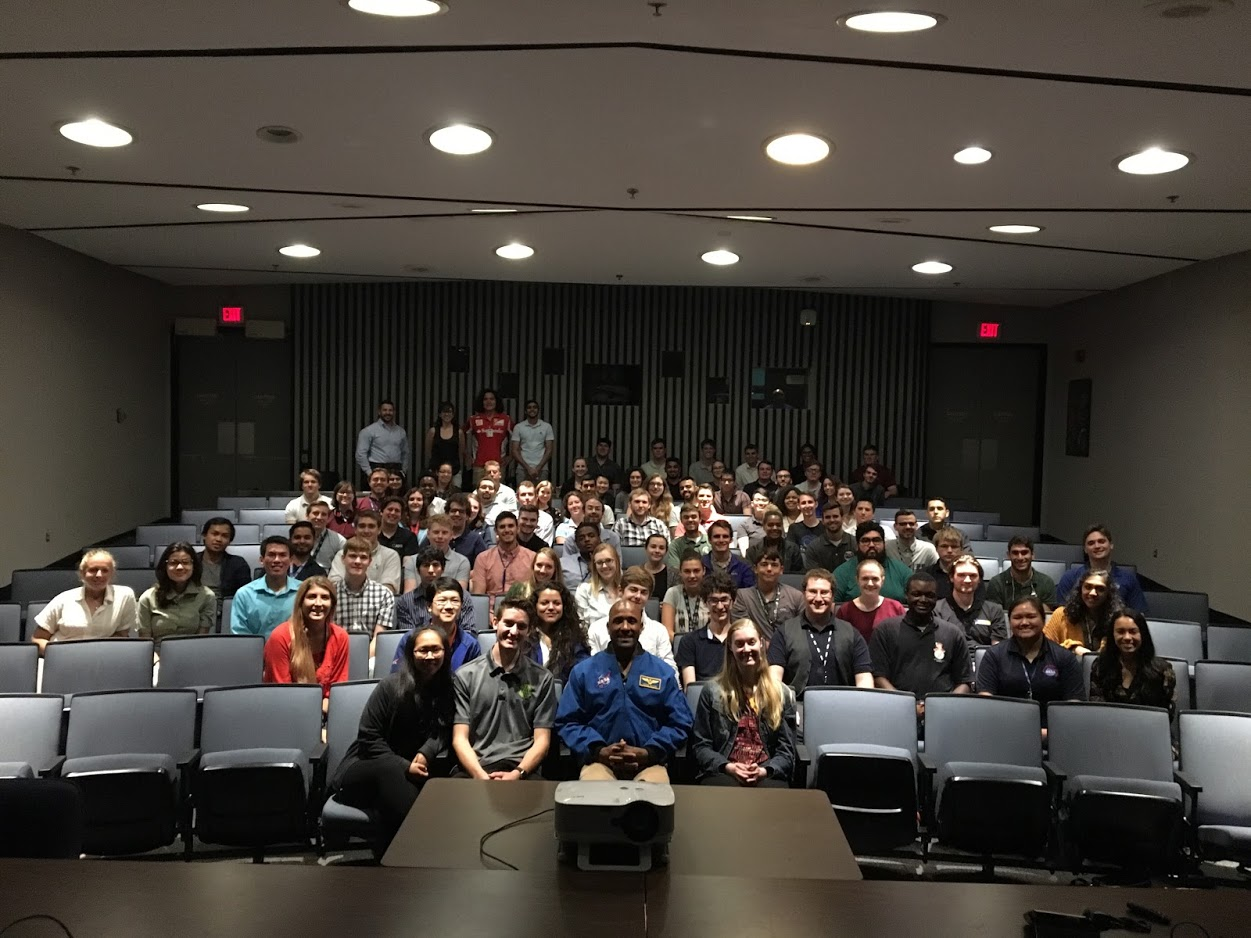
\includegraphics[width=0.75\textwidth]{assets/smalleroutreachgroup.png}
  \caption{Victor Glover Lecture}
  \label{fig:smalleroutreachgroup}
\end{figure}

\begin{figure}[!htb]
  \centering
  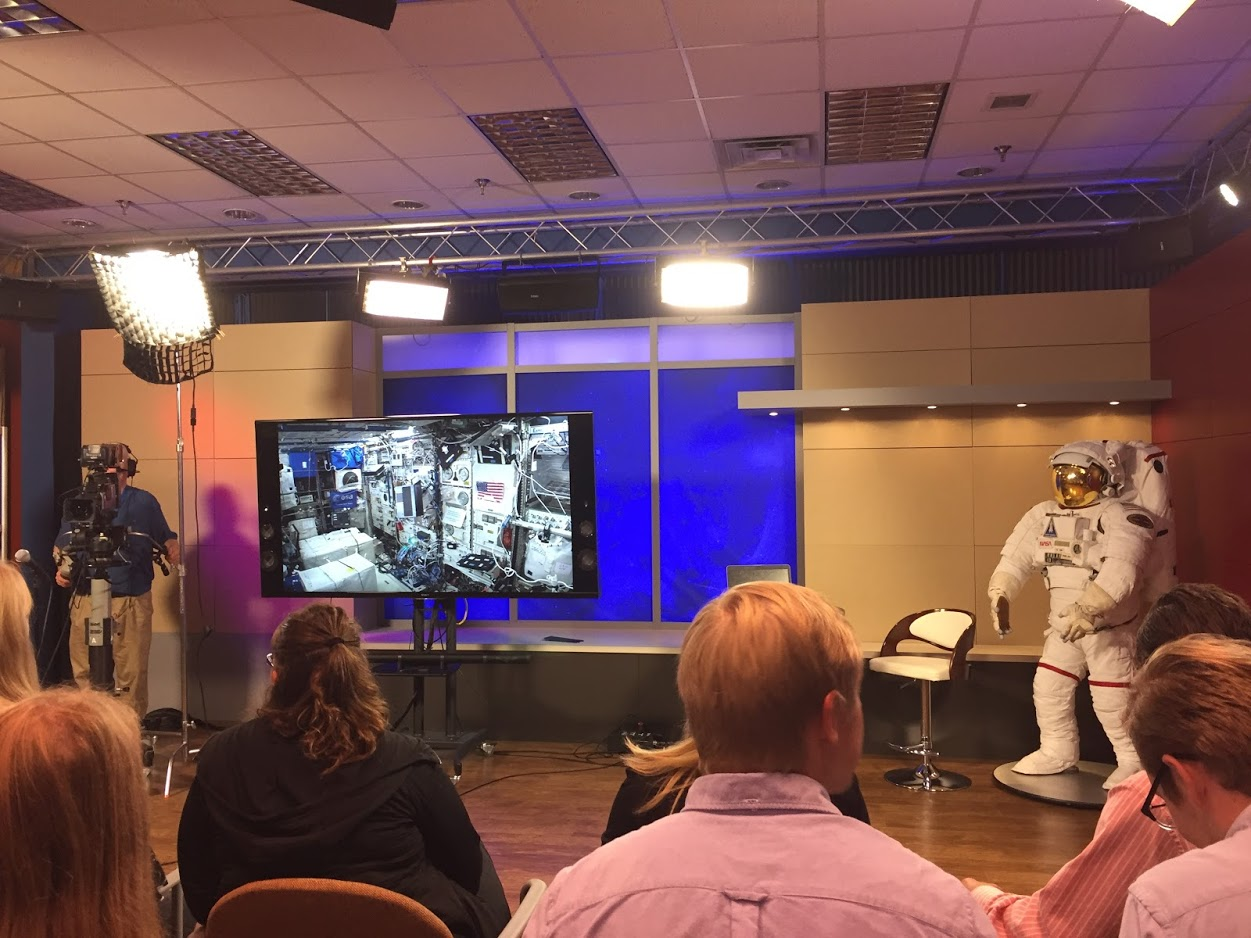
\includegraphics[width=0.75\textwidth]{assets/videodemonstration.png}
  \caption{ISS Downlink}
  \label{fig:videodemonstration}
\end{figure}

\begin{figure}[!htb]
  \centering
  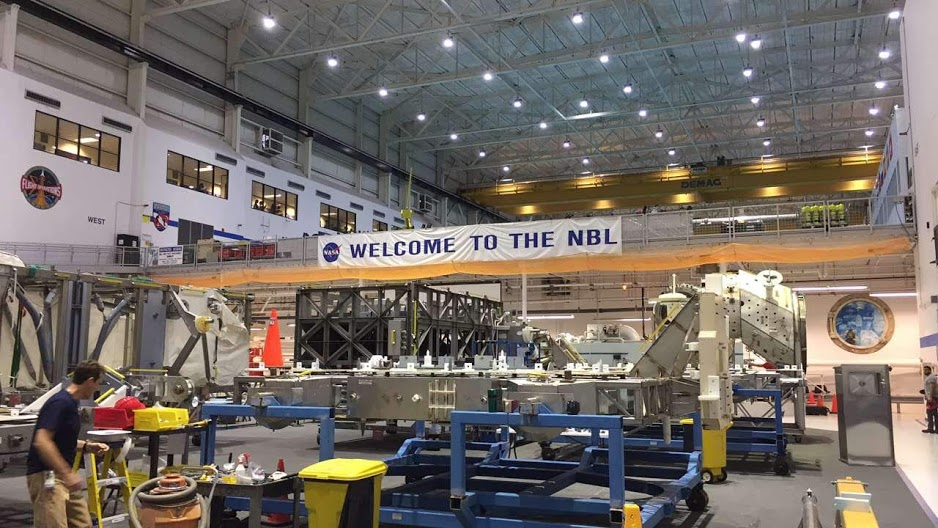
\includegraphics[width=0.75\textwidth]{assets/welcometonbl.png}
  \caption{Neutral Buoyancy Lab}
  \label{fig:welcometonbl}
\end{figure}

Above, \textit{Figure \ref{fig:videodemonstration}} and \textit{Figure \ref{fig:welcometonbl}} more of the amazing experiences working for NASA can provide. \textit{Figure \ref{fig:videodemonstration}} displays a live chat between interns and Astronaut Ricky Arnold on the International Space Station. \textit{Figure \ref{fig:welcometonbl}} shows one of the many impressive facilities NASA has to offer, both for tours and for serious research and training.

\begin{figure}[!htb]
  \centering
  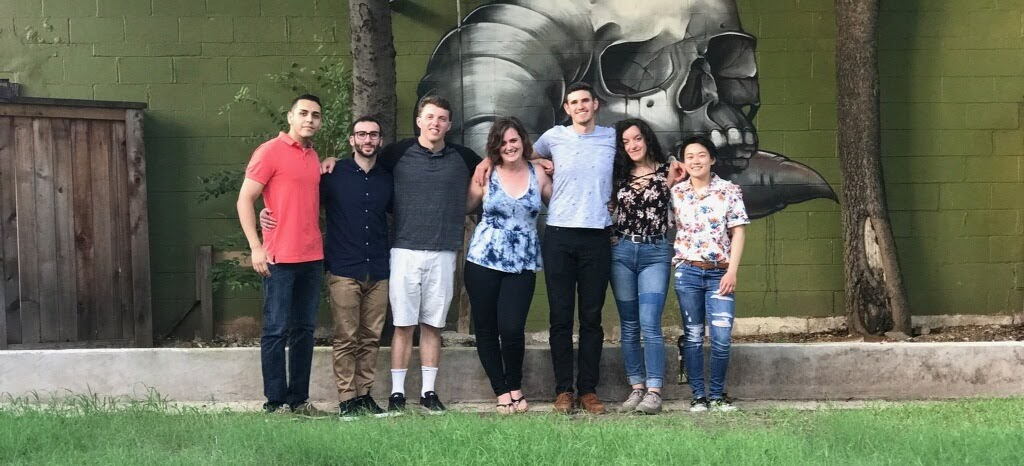
\includegraphics[width=0.75\textwidth]{assets/ronniewithfriends.png}
  \caption{Intern Family}
  \label{fig:ronniewithfriends}
\end{figure}

\begin{figure}[!htb]
  \centering
  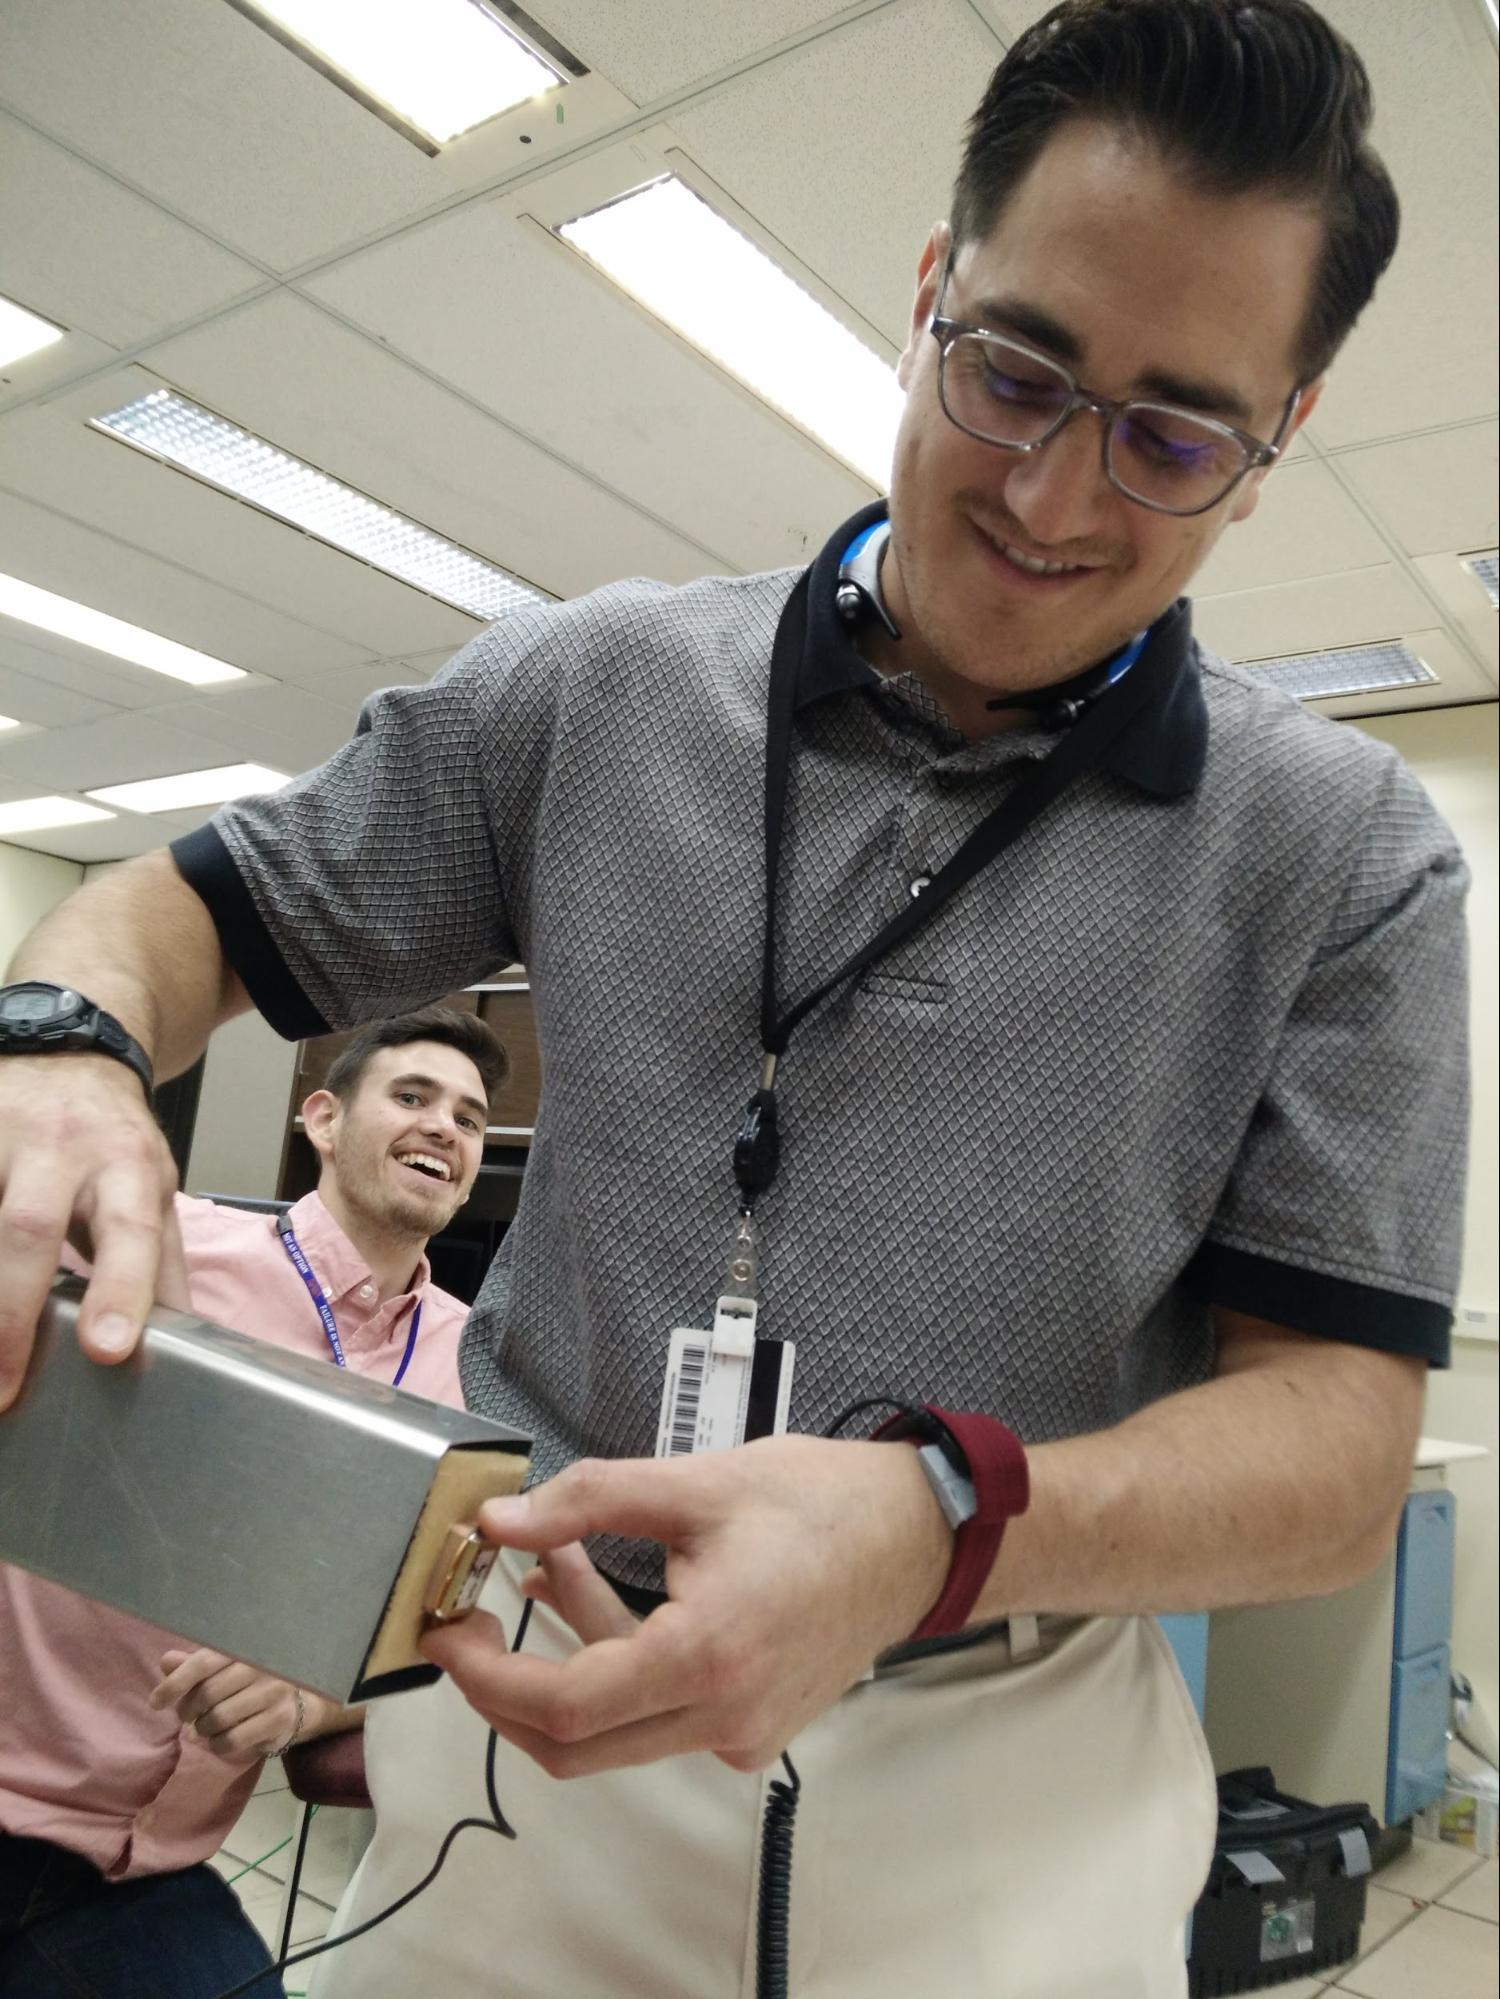
\includegraphics[width=0.5\textwidth]{assets/guywithpsu.jpg}
  \caption{Work Family}
  \label{fig:guywithpsu}
\end{figure}

Above all else though, NASA provides an incredible sense of family and community as shown in \textit{Figure \ref{fig:ronniewithfriends}} and \textit{Figure \ref{fig:guywithpsu}}.

\subsection{What you can provide to NASA}

In this section, we will go through our NASA Suits Project, its results, and our experience working on a NASA project while still in college. Hopefully at the point that we are presenting, we will have videos and pictures of a look forward to space and aeronautics in the next 30 years.

\subsection{Personal STEM / NASA Experiences}

Vincent Lee: EXPERIENCE DESCRIPTION

Joshua Schmidt: I have been involved in science and engineering for nearly my entire life. Since middle school in the gifted and talented program I have been programming and working with computer hardware, experimenting with OCR, networking, ML, and emerging technologies on various platforms. In highschool I was captain of my First robotics team, working closely with the design and programming divisions to create amazing robots. Now in Stevens I am working as a teaching assistant in intro to computer science. I do freelance work building web and native apps, and this past summer worked for Colgate-Palmolive developing their cloud infrastructure on GCP. I recently took a position at L3 technologies building communications and encryption software starting in the Spring. And I am a Computer Engineering major, pursuing a minor (possibly a major) in Computer Science.

Ian Pizzolo: One of my most memorable engineering experiences was back in a high school engineering class. I was in a class of about 25 students each split into 5 different teams. Each group was tasked with designing a vertical farming system. The system needed to be composed of multiple parts to be fabricated by each group. Each group made a design and the class voted on the design to be built. The design my group made was chosen and I was made the project leader. I delegated each part of the system to the 5 groups and made sure everyone stayed on task to complete the project. This developed my communication and leadership skills. This event also helped me make my decision to pursue engineering. Working with or for NASA has always been a dream of mine. NASA is on the front of aerospace technology and continue to lead the way and set the standards for others.

Ronnie Ankner: EXPERIENCE DESCRIPTION

\begin{figure}[!htb]
  \centering
  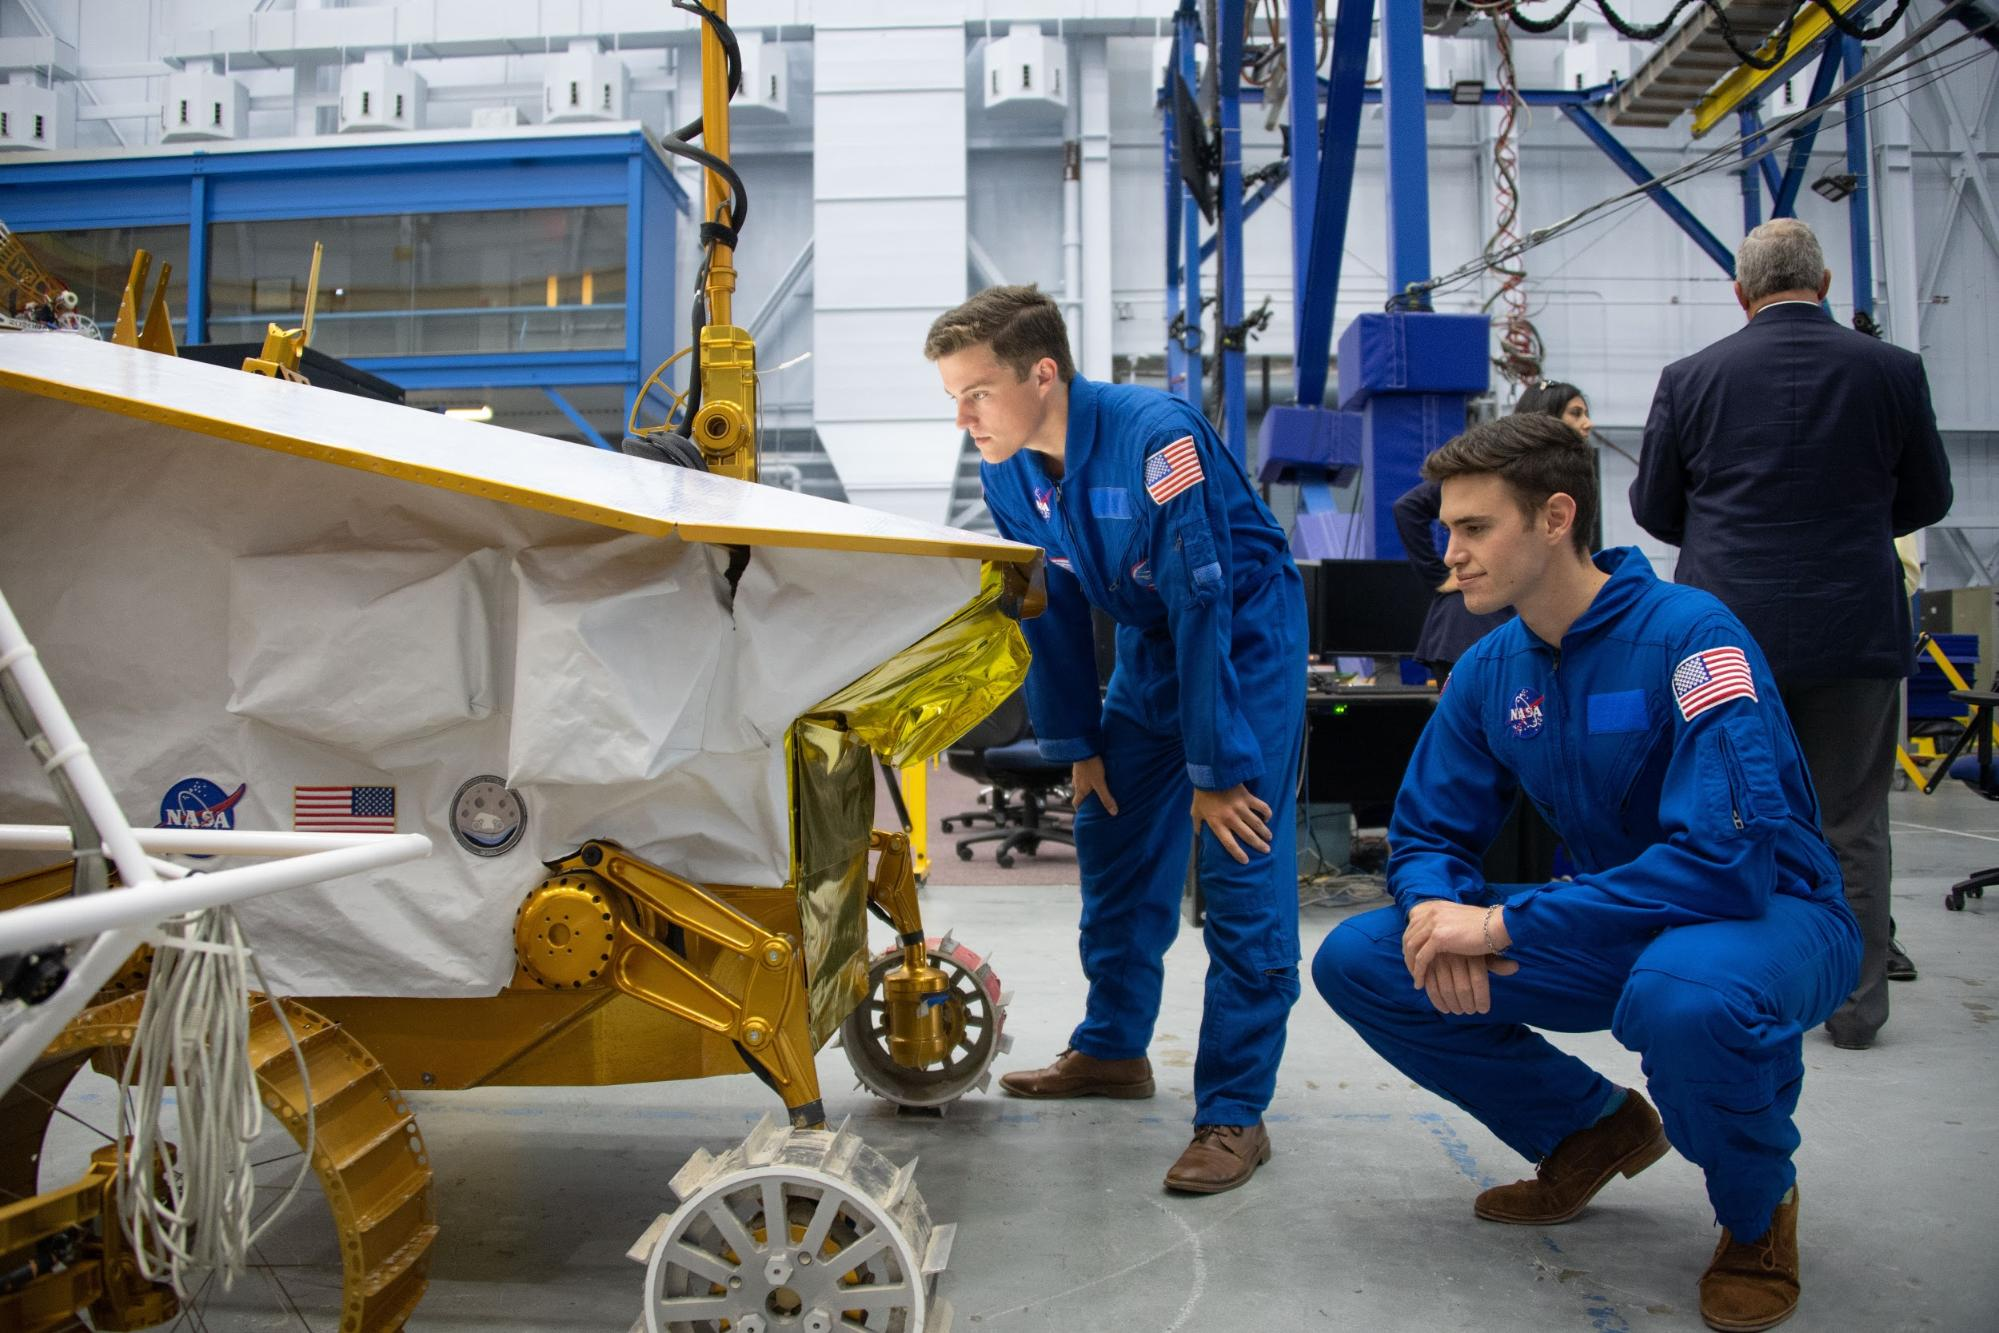
\includegraphics[width=0.75\textwidth]{assets/staringatrover.jpg}
  \caption{Day-in-the-life of an Astronaut 1}
  \label{fig:staringatrover}
\end{figure}

\begin{figure}[!htb]
  \centering
  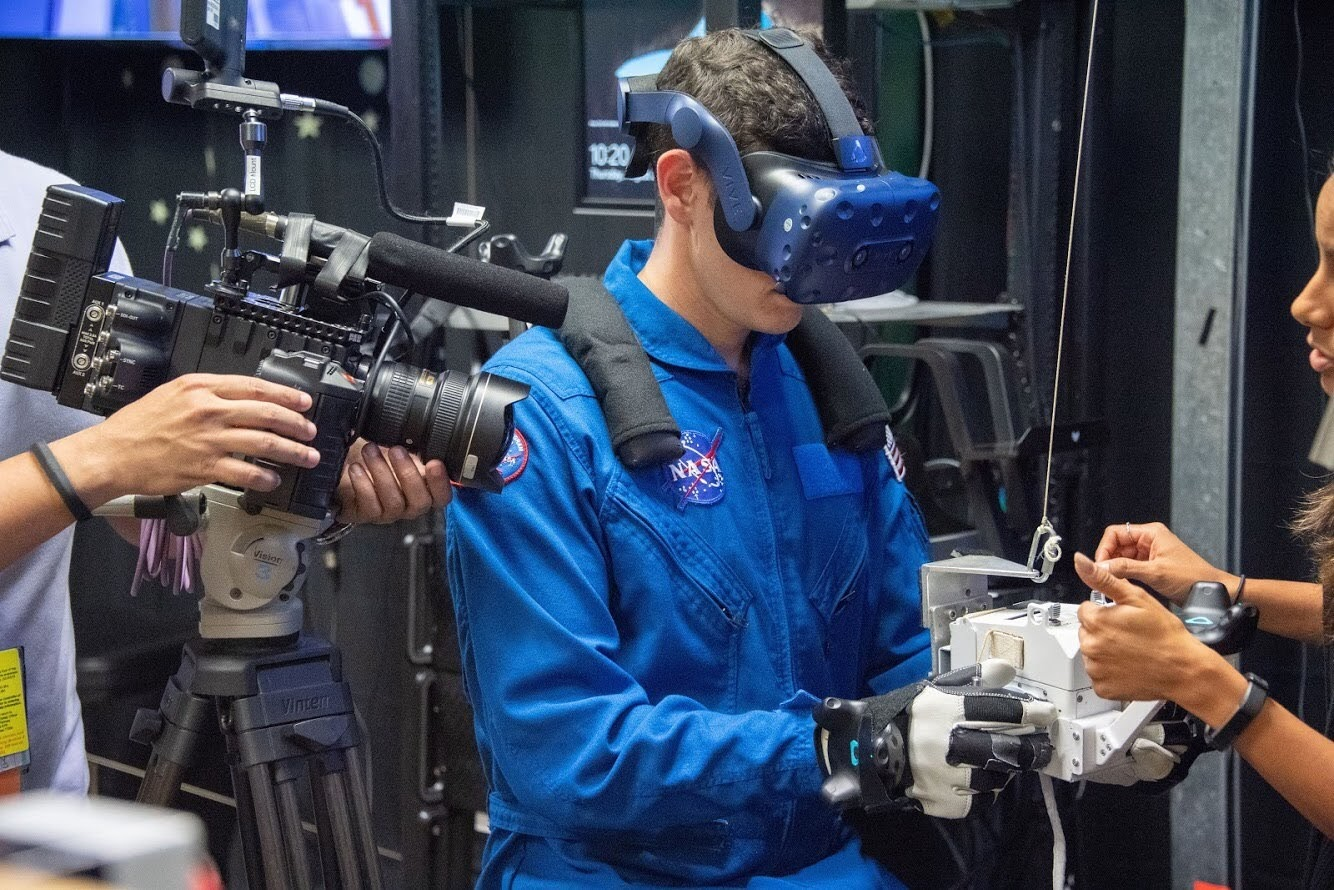
\includegraphics[width=0.75\textwidth]{assets/vrtest.png}
  \caption{Day-in-the-life of an Astronaut 2}
  \label{fig:vrtest}
\end{figure}

\begin{figure}[!htb]
  \centering
  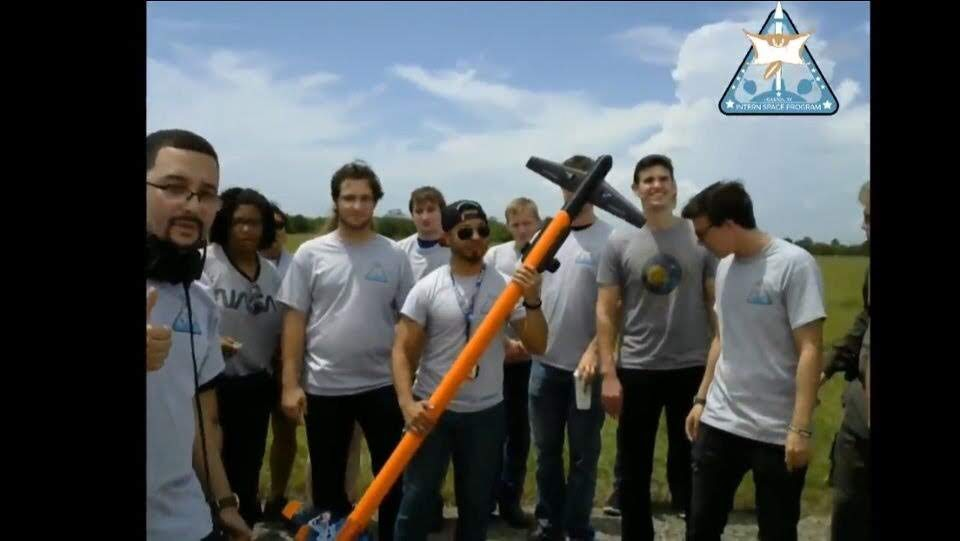
\includegraphics[width=0.75\textwidth]{assets/ronnieandplane.png}
  \caption{Intern Space Program}
  \label{fig:ronnieandplane}
\end{figure}

\subsection{Swag and Questions}

This section is relatively explanatory. We will open the floor to any and every question, offering select NASA “swag” for those brave enough to start the conversation. Furthermore, after the questioning period ends, we will stay longer and hear out individual questions, while also handing out the rest of the swag we have. 

We plan on visiting high schools in Hoboken as well as previous high schools that we have attended. Attached is a letter from Wayne Hills high school expressing interest in a presentation given by us to students that will encourage them to explore the field of stem. This system of outreach would, in our opinion, prove the most effective as high schoolers who have ambition in pursuing stem aren’t really introduced to ways to pursue outside of academics and therefore a presentation encouraging NASA and specific ways to get involved in STEM would definitely help usher the new generation in the right direction.

\newpage

\section{Administrative Section}

\subsection{Institutional Letter of Endorsement}

Ronnie do this

\newpage

\subsection{Statement of Supervising Faculty}

Someone needs to do this

\newpage

\subsection{Statement of Rights of Use}

As a team member for a proposal entitled “The First (Virtual) Man” proposed by a team of undergraduate students from Stevens Institute of Technology, I will and hereby do grant the U.S. Government a royalty free, nonexclusive and irrevocable license to use, reproduce, distribute (including distribution by transmission) to the public, perform publicly, prepare derivative works,and display publicly, any technical data contained in this proposal in whole or in part and in any manner for Federal purposes and to have or permit others to do so for
Federal purposes only. Further, with respect to all computer software designated by
NASA to be released as open source which is first produced or delivered under this
proposal and subsequent collaboration, if selected, shall be delivered with unlimited and
unrestricted rights so as to permit further distribution as open source. For purposes of
defining the rights in such computer software, “computer software” shall include source
codes, object codes, executables, ancillary files, and any and all documentation related
to any computer program or similar set of instructions delivered in association with this
collaboration. As a team member for a proposal entitled “The First (Virtual) Man” proposed by a team of undergraduate students from Stevens Institute of Technology, I will and hereby do
grant the U.S. Government a nonexclusive, nontransferable, irrevocable, paid-up
license to practice or have practiced for or on behalf of the United States Government
any invention described or made part of this proposal throughout the world.

\bigskip
\bigskip
\bigskip

\begin{tabular}{@{}p{.5in}p{3.5in}@{}}
Approved: & \hrulefill \\
& Anker, Ronald, 10/30/2018\\
\end{tabular}

\bigskip
\bigskip
\bigskip

\begin{tabular}{@{}p{.5in}p{3.5in}@{}}
Approved: & \hrulefill \\
& Lee, Vincent, 10/30/2018\\
\end{tabular}

\bigskip
\bigskip
\bigskip

\begin{tabular}{@{}p{.5in}p{3.5in}@{}}
Approved: & \hrulefill \\
& Pizzolo, Ian, 10/30/2018\\
\end{tabular}

\bigskip
\bigskip
\bigskip

\begin{tabular}{@{}p{.5in}p{3.5in}@{}}
Approved: & \hrulefill \\
& Schmidt, Joshua, 10/30/2018\\
\end{tabular}

\bigskip
\bigskip
\bigskip

\begin{tabular}{@{}p{.5in}p{3.5in}@{}}
Approved: & \hrulefill \\
& Iyengar, Mukund, 10/30/2018\\
\end{tabular}

\end{document}
